\documentclass[11pt,a4paper,twoside]{article}

% You should not change the line above.
% Nor change any of the formating.

% At a minimum, you need to edit the preamble file for your name and project
% title. There are a lot of latex commands there you might find useful.
\usepackage[a4paper]{geometry}
\usepackage{amsfonts}
\usepackage{amsthm}
\usepackage{amsmath}
\usepackage{parskip}
\usepackage{mathrsfs}
\usepackage{graphicx}
\usepackage{amssymb}
\usepackage{xtab}

% You need to set the next two items. 
% If you title is long, you may need to adjust the spacing in titlepage.tex
\newcommand{\TheAuthor}{Billy Sumners}
\newcommand{\TheTitle}{Examples and Counterexamples in the Theory of Tangent Measures}

% uncomment exacly one of these
%\newcommand{\TheModule}{\bf MA4K8 Scholarly Report}
\newcommand{\TheModule}{\bf MA4K9 Dissertation}


% Leave the following two as is
\newcommand{\TheUni}{The University of Warwick}
\newcommand{\TheDept}{Mathematics Institute}

% Set the correct submission year, e.g. replace 2000 with 2017
\newcommand{\TheSubDate}{\monthyear \formatdate{5}{4}{2019}}

% The are a lot of things you might find useful and want to uncomment. 
% Most things you will want to uncomment or change will be near the top.

% standard maths symbols (you probably want to uncomment all of these)
% \newcommand{\Z}{\ensuremath{\mathbb{Z}}}% integers
% \newcommand{\N}{\ensuremath{\mathbb{N}}}% natural numbers
% \newcommand{\R}{\ensuremath{\mathbb{R}}}% real numbers
% \newcommand{\C}{\ensuremath{\mathbb{C}}}% complex numbers

% Others 
%\newcommand{\st}{\ensuremath{:}}% such that
%\newcommand{\Tau}{\ensuremath{\mathcal{T}}}
%\newcommand{\Nat}{\mathbb{N}}

%\usepackage[numbers]{natbib}% round braces, sort multiple citations
\usepackage{hyperref}% creates hypertext links in pdf files (natbib compatible)
\usepackage{setspace}
%\usepackage{fancyhdr}
%\usepackage{mathrsfs}
%\usepackage{textcomp}
%\usepackage{color}
%\usepackage{graphicx}
%\usepackage{framed}
% \usepackage{algorithmic}% format pseudocode
%\usepackage[vlined,boxed,commentsnumbered,algochapter]{algorithm2e}
% \usepackage[chapter]{algorithm}% float wrapper for algorithms
%\usepackage{amsmath}% American Mathematical Society macros - essential!
%\usepackage{amssymb}% contains amsfonts
%\usepackage{amsthm}% allows more flexibility with theorems
\usepackage[nodayofweek]{datetime} % change the format of printed dates (no american style!) 
%\usepackage{ifdraft}% perform operations conditional on the draft option

%\usepackage{mathptmx}
% \usepackage{mathpazo}
%\usepackage{amscd}
% \usepackage{xy}
% \usepackage{diagxy}
%\usepackage{diagrams}

%\usepackage{marginnote}
%\usepackage{rotating}
%\usepackage{multirow}
% \usepackage{polski}
% \usepackage[T1]{fontenc}
% \usepackage{tikzpicture}
% \usetikzlibrary{matrix,arrows}

% \usepackage[inline]{showlabels}
%\usepackage{booktabs}

% Date format

% Use the datetime package
\newdateformat{monthyear}{\monthname[\THEMONTH], \THEYEAR}% new date format

% New commands, operators and symbols

% Operators
%\DeclareMathOperator{\Sym}{Sym}% symmetric group
%\DeclareMathOperator{\Alt}{Alt}% alternating group
%\DeclareMathOperator{\Id}{Id}
%\DeclareMathOperator{\Hom}{Hom}
%\DeclareMathOperator{\Grp}{Grp}
%\DeclareMathOperator{\supp}{supp}
%\DeclareMathOperator{\fix}{fix}
%\DeclareMathOperator{\dep}{dep}
%\DeclareMathOperator{\lcm}{lcm}
%\DeclareMathOperator{\Aut}{Aut}
%\DeclareMathOperator{\Inn}{Inn}
%\DeclareMathOperator{\Out}{Out}
% \DeclareMathOperator{\dim}{dim}
%\DeclareMathOperator{\Syl}{Syl}
%\DeclareMathOperator{\Hall}{Hall}
%\DeclareMathOperator{\pCore}{pCore}
%\DeclareMathOperator{\Char}{char}
%\DeclareMathOperator{\Image}{Im}
%\DeclareMathOperator{\Ker}{Ker}
%\DeclareMathOperator{\Hcf}{hcf}
%\DeclareMathOperator{\GL}{GL}
%\DeclareMathOperator{\Pc}{Pc}
%\DeclareMathOperator{\Stab}{Stab}
%\DeclareMathOperator{\Orbit}{Orbit}


% Hyphenation fixes
%\newcommand{\letdash}[1]{$#1$\nobreakdash-\hspace{0pt}}% for n-element, k-transitive etc
%\newcommand{\numdash}{\nobreakdash--}

% Sequences
%\newcommand{\seqfin}[3]{\ensuremath{#1_{#2}, \dotsc , #1_{#3}}}
%\newcommand{\seqinf}[3]{\ensuremath{#1_{#2}, #1_{#3}, \dotsc}}

% New environments

% Dedication
%\newenvironment{dedication}
%{\clearpage \thispagestyle{empty} \vspace*{\stretch{1}} \begin{center} \em}
%{\end{center} \vspace*{\stretch{3}} \clearpage}


% Page Layout

% Dimensions
% The guidlines for margins given by the Graduate School are as follows:
% left - no less than 4cm
% right - sufficient for trimming (?)
% top - no less than 1.5cm
% bottom - no less than 1.5cm
% See http://www2.warwick.ac.uk/services/academicoffice/gsp/current/presentation/
% Use the geometry package to set this up
\geometry{includehead,includefoot,left=3cm,right=3cm,top=2cm,bottom=2cm}% head and foot are included in total body so that nothing is printed out of the boundaries of the set margins

% Header and footer
% Use the fancydr package
%\ifdraft{%
%\fancypagestyle{plain}{% redefine plain pagestyle for draft
%\renewcommand{\headrulewidth}{0pt}% no head rule in draft mode
%\fancyhf{}% clear headers and footers
%\fancyhead[C]{\ifdraft{DRAFT}{}}% print DRAFT across top if the draft option is set
%\fancyfoot[C]{\thepage}% usual page numbering
%

%\pagestyle{fancy}
%\renewcommand{\chaptermark}[1]{\markboth{\thechapter.\ #1}{}}% compact with no capitalisation
%\renewcommand{\sectionmark}[1]{\markright{\thesection.\ #1}}% compact with no capitalisation
%\ifdraft{\renewcommand{\headrulewidth}{0pt}}{}% no head rule in draft mode
%\setlength{\headheight}{15pt}
%\fancyhf{}% clear all header and footer fields
% one-sided printing, so no E,O distinction need be made
%\fancyhead[C]{\ifdraft{DRAFT}{}}% print DRAFT across top if the draft option is set
%\fancyhead[R]{\thepage}% page in top right
%\fancyhead[L]{\ifdraft{}{\leftmark}}% chapter number and title in top left

% Theorems
%
%\newtheorem{prop}{Proposition}[chapter]
%\newtheorem{lemma}[prop]{Lemma}
%\newtheorem{conjecture}[prop]{Conjecture}
%\newtheorem{theorem}[prop]{Theorem}
%\newtheorem{hyp}[prop]{Hypothesis}
%\newtheorem{cor}[prop]{Corollary}
%\newtheorem{claim}[prop]{Claim}
%\newtheorem{remark}[prop]{Remark}
%\newtheorem{notation}[prop]{Notation}
%\newtheorem{defn}[prop]{Definition}


% Numbering
%\numberwithin{equation}{chapter}% standard style numbering, nothing special here


% Algorithms

% Use the algorithms package.
% \renewcommand{\algorithmicrequire}{\textbf{Input:}}
% \renewcommand{\algorithmicensure}{\textbf{Output:}}
% \renewcommand{\algorithmiccomment}[1]{/* #1 */}
%\RestyleAlgo{boxruled}
%\SetAlgoInsideSkip{medskip}
%\setlength{\algomargin}{2em}
%\setlength{\interspacetitleboxruled}{0.7em}
%\setlength{\interspacetitleruled}{0.7em}
%\LinesNumbered
%\SetAlCapNameSty{sc}
%\SetFuncSty{sc}

%\newenvironment{spacedalgorithm}{\begin{algorithm}\onehalfspacing}{\end{algorithm}}
% \newenvironment{onehalfverbatim}{\onehalfspacing\begin{verbatim}}{\end{verbatim}}

%\reversemarginpar
%\newcounter{nootje}
%\setcounter{nootje}{1}
%\renewcommand\check[1]{[*\thenootje]\marginnote{\tiny\begin{minipage}{40mm}\begin{flushright}\thenootje
%: #1\end{flushright}\end{minipage}}\addtocounter{nootje}{1}}


% Document details

\usepackage{times, mathptmx}
\usepackage{amsfonts, amsmath, amsthm, mathrsfs, enumitem, tensor}
\usepackage{bbm}
\usepackage{relsize}
%\usepackage[margin=3cm]{geometry}
\usepackage{tikz}
\usepackage{wrapfig}
\usepackage{xcolor} 
%\usepackage{times}
\usepackage[framemethod=tikz]{mdframed}
%\usepackage{biblatex}

%\bibliography{tangent_measures}

\newcommand{\bbR}{\mathbb{R}}
\newcommand{\bbN}{\mathbb{N}}
\newcommand{\bbQ}{\mathbb{Q}}
\newcommand{\bbP}{\mathbb{P}}
\newcommand{\bbone}{\mathbbm{1}}

\newcommand{\scrA}{\mathscr{A}}
\newcommand{\scrB}{\mathscr{B}}
\newcommand{\scrL}{\mathscr{L}}
\newcommand{\scrH}{\mathscr{H}}
\newcommand{\scrQ}{\mathscr{Q}}
\newcommand{\scrS}{\mathscr{S}}
\newcommand{\scrR}{\mathscr{R}}

\renewcommand{\epsilon}{\varepsilon}
\renewcommand{\phi}{\varphi}

\newcommand{\abs}[1]{\left\vert {#1} \right\vert}
\newcommand{\norm}[1]{\left\Vert {#1} \right\Vert}
\newcommand{\set}[1]{\left\{ {#1} \right\}}
\newcommand{\parens}[1]{\left( {#1} \right)}

\newcommand{\restrict}{\begin{picture}(10,8)\put(2,0){\line(0,1){7}}\put(1.8,0){\line(1,0){7}}\end{picture}}
\newcommand{\restrictsmall}{\begin{picture}(7,6)\put(1,0){\line(0,1){6}}\put(0.8,0){\line(1,0){6}}\end{picture}}  

\newcommand{\bigllcorner}{\mathlarger{\llcorner}}

\newcommand{\weakstar}{\overset{\ast}{\rightharpoonup}}
\newcommand{\wslim}{\operatorname{w*-lim}} 
 
\newcommand{\Tan}{\operatorname{Tan}}
\newcommand{\supp}{\operatorname{supp}}
\newcommand{\Flat}{\operatorname{Flat}}

\newcommand{\scrM}{\mathscr{M}}

\renewcommand{\d}[1]{\ensuremath{\operatorname{d}\!{#1}}} 
\renewcommand{\O}{\mathrm{O}}
\newcommand{\T}{\mathrm{T}}
\newcommand{\J}{\mathrm{J}}

\renewcommand{\qedsymbol}{\includegraphics{slamdunk.jpg}}

\DeclareMathOperator{\Lip}{Lip}

\theoremstyle{plain}
\newtheorem{theorem}{Theorem}[section]
\newtheorem{lemma}[theorem]{Lemma}
\newtheorem{proposition}[theorem]{Proposition}
\newtheorem{corollary}[theorem]{Corollary}
\newtheorem{question}[theorem]{Question}

\theoremstyle{definition}
\newtheorem{example}[theorem]{Example}

\theoremstyle{remark}
\newtheorem{remark}[theorem]{Remark}

\numberwithin{equation}{section}

\surroundwithmdframed[outerlinewidth=0.4pt,middlelinewidth=1pt,innerlinewidth=0.4pt,middlelinecolor=white,bottomline=false,topline=false,rightline=false,skipabove=10pt,innerbottommargin=-1pt]{theorem}
\surroundwithmdframed[outerlinewidth=0.4pt,bottomline=false,topline=false,rightline=false,skipabove=10pt,innerbottommargin=-1pt]{lemma}
\surroundwithmdframed[outerlinewidth=0.4pt,bottomline=false,topline=false,rightline=false,skipabove=10pt,innerbottommargin=-1pt]{proposition}
\surroundwithmdframed[outerlinewidth=0.4pt,bottomline=false,topline=false,rightline=false,skipabove=10pt,innerbottommargin=-1pt]{corollary}
%\surroundwithmdframed[outerlinewidth=0.4pt,bottomline=false,topline=false,rightline=false,skipabove=10pt,innertopmargin=12pt]{question}
%\surroundwithmdframed[tikzsetting={draw=black,line width=1pt,dashed},bottomline=false,topline=false,rightline=false,outerlinecolor=white,middlelinecolor=white,skipabove=10pt,innertopmargin=12pt]{example}


\begin{document}
 
\pagenumbering{roman}
\include{titlepage}
\setcounter{page}{2}
\include{contents}
\onehalfspacing
\pagenumbering{arabic}
\onehalfspacing
\raggedbottom

% Now starts the main part of the report. 
% Each section/chapter is in a separate file. Two examples are include.
% 
% This part (between TOC and Bibliograpy) must obey:
% for MA4K8 must not exceed 30 pages.
% for MA4K9 the target is approx 30 pages and must not exceed 40 pages.

\section{Introduction}
Given a smooth submanifold $M \subseteq \bbR^d$, we know how its tangent space $T_pM$ at a point $p \in M$ is defined, and what it represents. Namely, $T_p M$ should represent the ``best linear approximation'' to $M$ near $p$, much like the derivative of a differentiable function represents its best linear approximation near a point. Although $T_p M$ is usually defined via quite abstract methods, the situation of being a subset of Euclidean space allows us to interpret $T_p M$ in the very concrete sense of ``zooming in'' to $p$, or ``blowing up'' the manifold $M$ around $p$. Such a procedure is applicable to far more general subsets of $\bbR^d$, and can often lead to more interesting results than a simple vector space. Typically, this ``tangent cone'' is denoted $\Tan(M,p)$ See figure \ref{fig:blowingUpCorner} for an example of a set whose tangent cone at a point is not an affine subspace of $\bbR^d$.

It turns out that this blowup procedure applies to measures on $\bbR^d$, and is related to blowing up subsets of $\bbR^d$ in the sense that if $M \subseteq \bbR^d$ is an $m$-dimensional submanifold of $\bbR^d$, blowing up the $m$-dimensional Hausdorff  measure on $M$ (which we denote $\scrH^m \restrict M$) at a point $p \in M$ gives us $\scrH^m \restrict T_pM$. In section \ref{sec:submanifolds}, we will see this in a more rigorous setting. Now, measures on $\bbR^d$ are far more numerous than subsets of $\bbR^d$, so we would like to ask how much worse can this blowup procedure for measures be compared to blowing up subsets of $\bbR^d$? It turns out that the answer is ``a lot worse''. In the following project, we will demonstrate the existence of a measure on $\bbR^d$ such that, at almost every point in its support,, we can adjust the speed of blowing up to give us any measure imaginable on $\bbR^d$. As somewhat of a converse, we will also construct a measure on $\bbR$ which looks completely unlike Lebesgue measure on $\bbR$ (think a countable sum of $\delta$ measures), but blowing up at almost every point in its support returns Lebesgue measure.

\begin{figure} \label{fig:blowingUpCorner}
    \centering
    \begin{tikzpicture}
        %\draw[gray] (-1,-1) grid (10,3);

        \draw[blue] (0,1) node[left,color=black] {$p$} .. controls (1.25,1.25) and (1.75,1.75) .. (1.5,2.5);
        \filldraw[red] (0,1) circle (0.05);
        \draw[blue] (0,1) .. controls (0.25,0.25) and (1,0) .. (2,0);
        %\draw[red] (0,1) circle (0.25);
        \node (M) at (1,-0.5) {$M$}; 

        \draw[->] (2.5,1) -- (3.25,1) node[align=center,above] {blowup} -- (4,1);

        \draw[blue] (4.5,1.5) -- (6,2.0);
        \draw[blue] (4.5,1.5) -- (5.25,0);
        \node (TpM) at (5,-0.5) {$\Tan(M,p)$};
    \end{tikzpicture}

    \caption{Blowing up a corner}
\end{figure}

\section{Tangent Measures}
\subsection{Blowing up and Tangent Measures} \label{sec:blowingUp}
To formalize the notion of ``blowing up'' a measure, fix $p \in \bbR^d$ and $r > 0$. Define the homothety $T^{p,r} \colon \bbR^d \to \bbR^d$ by 
\begin{equation}
    T^{p,r}(x) := \frac{x - p}{r}.
\end{equation}
Under this map, the ball $B(p,r)$ gets mapped to $B(0,1)$ (See figure \ref{fig:homothety}). Given $\mu \in \scrM(\bbR^d)$, we define the \textit{pushforward} $\mu_{p,r} = T^{p,r}_*\mu$ of $\mu$ by
\begin{equation}
    \mu_{p,r}(A) = \mu((T^{p,r})^{-1}(A)) = \mu(p + rA) \quad \text{for } A \subseteq \bbR^d \text{ a Borel set.}
\end{equation}
Suppose now there exists a sequence $r_j > 0$ with $r_j \downarrow 0$ as $j \rightarrow \infty$ and sequence $c_j > 0$ of normalizing constants such that $c_j \mu_{p,r_j}$ converges weakly* to some $\tau \in \scrM(\bbR^d)$. We then call $\tau$ a \textit{tangent measure} to $\mu$ at $p$, and $c_j \mu_{p,r_j}$ a \textit{blowup sequence} for $\tau$. We write $\Tan(\mu,p)$ for the set of all tangent measures to $\mu$ at $p$.

\begin{figure} 
    \centering
    \begin{tikzpicture}
        %\draw[gray] (0,0) grid (10,5);

        \node[anchor = south west] (mona) at (1,1) {\includegraphics[height=3cm]{monaLisa.jpg}};
        \draw[red, thick] (2.3,3.5) circle (0.2);
        \node (monazoom) at (8.1,2.6) {\includegraphics[height=3cm]{monaLisaZoom.jpg}};
        \draw[red,thick] (8,2.3) circle (0.8);

        \draw[->] (4,2.5) to[out=30,in=150] (6,2.5);
        \node (T) at (5,3.1) {$T^{p,r}$};
    \end{tikzpicture}
    \caption{The homothety $T^{p,r}$.}
    \label{fig:homothety}
\end{figure}

We remark that the above definition does not need $\mu$ or $\tau$ to be positive measures at all, and works perfectly well for signed (or even vector-valued) measures.

The structure of $\Tan(\mu,p)$ is of some interest, and we will be making use of the following lemma later.
\begin{lemma} \label{lem:tangent_measure_properties}
    Fix $\mu \in \scrM(\bbR^d)$ and $p \in \bbR^n$. Suppose $\tau \in \Tan(\mu,x_0)$. Then
    \begin{enumerate}[label={\rm (\alph*)}]
        \item For all $c > 0$, the measure $c\tau$ is in $\Tan(\mu,p)$.
        \item For all $r > 0$, the measure $\tau_{0,r}$ is in $\Tan(\mu,p)$.
        \item The set $\Tan(\mu,p)$ is closed in $\scrM(\bbR^d)$ (with respect to the weak* topology). 
    \end{enumerate}
\end{lemma}
\begin{proof}
    Let $c_j \mu_{p,r_j}$ be a blowup sequence for $\tau$. Then $c c_j \mu_{p,r_j}$ is a blowup sequence for $c\tau$, which can be easily checked. Similarly, $c_j \mu_{p,rr_j}$ is a blowup sequence for $\tau_{0,r}$. Indeed, given $\psi \in C_c(\bbR^d)$, we have
    \begin{equation}
        \int_{\bbR^d} c_j \phi \; \d{\mu_{p,rr_j}} = \int_{\bbR^d} c_j \phi\left( \frac{1}{r}\frac{x-p}{r_j} \right) \; \d{\mu(x)}
                                           \rightarrow \int_{\bbR^d} \phi\left( \frac{x}{r} \right) \; \d{\tau(x)}
                                                     = \int_{\bbR^d} \phi \; \d{\tau_{0,r}}.
    \end{equation}
    This proves (a) and (b).

    To prove (c), let $d$ be a metric on $\scrM(\bbR^d)$ generating the weak* topology (see lemma \ref{lem:metrizabilityofWeak*Convergence}).
    Let $\tau^{(n)}$ be a sequence in $\Tan(\mu,p)$ converging to $\tau \in \scrM(\bbR^d)$, and take a blowup sequence $c_j^{(n)}\mu_{p,r_j^{(n)}}$ for each $n \in \bbN$. We need to find a blowup sequence $\overline{c}_j \mu_{p,\overline{r}_j}$ converging to $\tau$.
    
    We do this construction inductively. Initially, take $n_1 = j_1 = 1$. Given $m \in \bbN$, assume that $n_{m-1}$ and $j_{m-1}$ have been found, and choose $j_m > j_{m-1}$ such that $d(\tau^{(n_m)},\tau) < \frac{1}{2m}$, and $j_m > j_{m-1}$ such that $d(c_{j_m}^{(n_m)}\mu_{p,r_{j_m}^{(n_m)}},\tau^{(n_m)}) < \frac{1}{2m}$ and $r_{j_m}^{(n_m)} < \min\left( r_{j_{m-1}}^{(n_{m-1})},\frac{1}{m} \right)$ (which is always possible since $r_j^{(n_m)} \downarrow 0$ as $j \to \infty$ by definition of a blowup sequence). Define $\overline{c}_m := c^{(n_m)}_{j_m}$ and $\overline{r}_m := r^{(n_m)}_{j_m}$. Then 
    \begin{equation}
        d(\overline{c}_m \mu_{p,\overline{r}_m}, \tau) \leq d(\overline{c}_m \mu_{p,\overline{r}_m}, \tau^{(j_m)}) + d(\tau^{(j_m)},\tau)
                                                          < \frac{1}{2m} + \frac{1}{2m}
                                                          = \frac{1}{m},
    \end{equation}
    which shows that $\overline{c}_m \mu_{p,\overline{r}_m} \weakstar \tau$ as $m \to \infty$. By construction, we have that $\overline{r}_m \downarrow 0$ as $m \to \infty$, and so $\overline{c}_m \mu_{p,\overline{r}_m}$ is a legitimate blowup sequence for $\tau$. It follows that $\tau \in \Tan(\mu,p)$, thereby proving (c).
\end{proof}
In the language of [Preiss], properties (a) and (b) of the above lemma say $\Tan(\mu,p)$ is a $d$-cone. In general, $\Tan(\mu,p)$ is not a vector space.

The above lemma will help us to show that the normalizing constants $c_j$ aren't so important. Indeed, suppose $c_j \mu_{p,r_j}$ is a blowup sequence for $\tau \in \Tan(\mu,p)$. Let $K > 0$ be such that $\tau(B(0,K)) > 0$, and define $\widetilde{c}_j := \mu(B(p,Kr_j))^{-1}$. Then by semicontinuity (lemma \ref{lem:semicontinuityOfWeak*Convergence}),
\begin{equation} \begin{aligned}
    0 < \tau(B(p,K)) &\leq \liminf_{j \to \infty} c_j \mu_{p,r_j}(B(0,K)) \\
                     &= \liminf_{j \to \infty} c_j \mu(B(p,Kr_j)) \\
                     &\leq \limsup_{j \to \infty} c_j \mu(\overline{B(p,Kr_j)}) \\
                     &= \limsup_{j \to \infty} c_j \mu_{p,r_j}(\overline{B(0,K)}) \\
                     &\leq \tau(\overline{B(0,K)}) < \infty,
\end{aligned} \end{equation}
since $\tau$ is a Radon measure. Pass to a subsequence such that $c_j\mu(B(p,Kr_j))$ converges to a positive value $c$. It follows that 
\begin{equation}
    \widetilde{c}_j \mu_{p,r_j} = \frac{\widetilde{c}_j}{c_j} c_j \mu_{p,r_j} \weakstar c \tau.
\end{equation}
So $\widetilde{c}_j \mu_{p,r_j}$ is a blowup sequence for $c \tau$. Dividing by $c$, we see $c^{-1}c_j \mu_{p,r_j}$ is a blowup sequence for $\tau$.

Another simple property of $\Tan(\mu,p)$ is that it is nonempty: we can take $c_j = 0$ for all $j$ to see that $0$ is a tangent measure to any $\mu$ at any point $p \in \bbR^d$. Is $\Tan(\mu,p)$ nonzero in general? It turns out that it is for $\mu$-a.e. $p \in \bbR^d$ - see {\bf [Rindler prop 10.5]} for a proof.

\subsection{Examples of Tangent Measures and their Local Properties} \label{sec:examplesAndLocal}
Fix $p \in \bbR^d$. Consider $\mu = \scrL^d$, and fix $\phi \in C_c(\bbR^d)$. Then
\begin{equation} \begin{aligned}
    \int_{\bbR^d} \phi \; \d(r^d \mu_{p,r}) &= \int_{\bbR^d} \phi\left( \frac{x-p}{r} \right) r^d \; \d\scrL^d(x) \\
                                                &= \int_{\bbR^d} \phi(y) r^d r^{-d} \; \d\scrL^d(y)                     \\
                                                &= \int_{\bbR^d} \phi \; \d\scrL^d,
\end{aligned} \end{equation}
where we made the change of variables $y = r^{-1}(x-p)$. It follows that for any sequence $r_j \downarrow 0$, the sequence $r_j^{-d} \mu_{x_0,r_j}$ is a blowup sequence for $\scrL^d$, and therefore $\scrL^d$ is a tangent measure to itself at $p$

More generally, let $f \in C(\bbR^d)$ be nonnegative, define $\mu = f \scrL^d$, and fix $\phi \in C_c(\bbR^d)$. Similarly to above, we find 
\begin{equation} \begin{aligned}
    \int_{\bbR^d} \phi \; \d(r^{-d} \mu_{p,r}) &= \int_{\bbR^d} \phi\left( \frac{x-p}{r} \right) f(x) r^{-d} \; \d\scrL^d(x) \\
                                                    &= \int_{\bbR^d} \phi(y) f(p + ry) \; \d\scrL^d(y)                            \\
                                                    &\rightarrow \int_{\bbR^d} \phi(y) f(p) \; \d\scrL^d(y).
\end{aligned} \end{equation}
Where we again made the change of variables $y = r^{-1}(x-x_0)$, and used the dominated convergence theorem together with the fact that $\phi$ and $f$ are continuous functions, and $\phi$ has compact support. We see that $f(p) \scrL^d$ is a tangent measure to $f \scrL^d$ at $p$.

The above situation is true for far more measures than just Lebesgue measure. Let $f \in C(\bbR^d)$ be nonnegative, fix $\mu \in \scrM(\bbR^d)$, and consider the measure $f\mu$. Fix $\phi \in C_c(\bbR^d)$, and let $R > 0$ be such that $\supp{\phi} \subseteq B(0,R)$. Choose a tangent measure $\tau \in \Tan(\mu,p)$ and a blowup sequence $c_j \mu_{p,r_j}$ for $\tau$. Then 
\begin{equation} \begin{aligned}
    \int_{\bbR^d} c_j \phi \;\d(f\mu)_{p,r_j} &= \int_{\bbR^d} c_j \phi\parens{\frac{x-p}{r_j}} f(x) \; \d\mu(x) \\
                                                &= \int_{\bbR^d} c_j \phi\parens{\frac{x-p}{r_j}} f(p) \; \d\mu(x) \\
                                                &\quad + \int_{\bbR^d} c_j \phi\parens{\frac{x-p}{r_j}} ( f(x) - f(p) ) \; \d\mu(x).
\end{aligned} \end{equation}
The first term converges to
\begin{equation}
    \int_{\bbR^d} \phi(x) f(p) \; \d\tau(x).
\end{equation}
For the second term, note that $x \mapsto \phi\parens{\frac{x-p}{r_j}}$ is supported in $B(p, Rr_j)$, so the magnitude of the second term is bounded by some constant (independent of $x$ and $r_j$) times
\begin{equation}
    \sup_{x \in B(p,Rr_j)} \abs{f(x) - f(p)}.
\end{equation}
Now, $f$ is uniformly continuous on $B(p,R)$, so this term converges to zero as $j \to \infty$. It follows that $f(p) \tau$ is a tangent measure to $f\mu$ at $p$. In particular, $f(p)\Tan(\mu,p) \subseteq \Tan(f\mu,p)$

We would now like to show the converse inclusion holds: if $\tau$ is a tangent measure to $f\mu$ at $p$, then $\tau = f(p) \widetilde{\tau}$ for some $\widetilde{\tau} \in \Tan(\mu,p)$. Let $c_j (f\mu)_{p,r_j}$ be a blowup sequence for $\tau$. Then, for all $\phi \in C_c(\bbR^d)$, we have 
\begin{equation} \begin{aligned}
    \int_{\bbR^d} \phi \; \d\tau &= \lim_{j \to \infty} \int_{\bbR^d} \phi \; \d(c_j (f \mu)_{p,r_j}) \\
                                 &= \lim_{j \to \infty} \int_{\bbR^d} c_j \phi\parens{ \frac{x-p}{r_j} } f(x) \; \d\mu(x) \\
                                 &= \lim_{j \to \infty} \int_{\bbR^d} c_j \phi\parens{ \frac{x-p}{r_j} } f(p) \; \d\mu(x) \\
                                 &\quad + \lim_{j \to \infty} \int_{\bbR^d} c_j \phi\parens{ \frac{x-p}{r_j} } (f(x) - f(p)) \; \d\mu(x).
\end{aligned} \end{equation}
The same argument as above implies the second term is zero. If $f(p) > 0$, take $\widetilde{\tau} = f(p)^{-1} \tau$. We then see that $\widetilde{\tau}$ is a tangent measure to $\mu$ at $p$ with blowup sequence $c_j \mu_{p,r_j}$. If $f(p) = 0$, it follows immediately that $\tau = 0$, so we can take $\widetilde{\tau}$ to be any tangent measure of $\mu$ (for example, $\widetilde{\tau} = 0$). We have shown that $\Tan(f\mu,p) = f(p)\Tan(\mu,p)$.

By an approximation argument, it can be shown that for any $f \in L^1(\bbR^d)$ and $\mu$-a.e. $p \in \bbR^d$, the property $\Tan(f\mu,p) = f(p) \Tan(\mu,p)$ is true {\bf [de lellis]}. In particular, for any Borel measurable subset $A \subseteq \bbR^d$ containing $p$, we can take $f = \bbone_A$ to show that $\Tan(\mu \restrict A,p) = \Tan(\mu,p)$ for $\mu$-a.e. $p \in A$. This property captures the intuition that tangent measures should be a local property of measures.

%The following example is a baby version of the O'Neil measure we consider later. Set $s_i := 2^{-i+1}$ and $\widetilde{s}_i := -3^{-i+1}$ for $i \in \bbN$. Define 
%\begin{equation}
%    \mu := \sum_{i=1}^\infty \frac{\delta_{s_i} + \delta_{\widetilde{s}_i}}{2^i}.
%\end{equation}
%Fix $\phi \in C_c(\bbR)$ as usual. For $r_j = s_j$, we have 
%\begin{equation} \begin{aligned}
%    \int_{\bbR} \phi \; \d(2^j\mu_{0,r_j}) &= \int_{\bbR} \phi\left( \frac{x}{r_j} \right) 2^j \; \d\mu                                               \\
%                                            &= \sum_{i=1}^\infty 2^{j-i} \left( \phi\left( \frac{s_i}{r_j} \right) + \phi\left( \frac{\widetilde{s}_i}{r_j} \right) \right) \\
%                                            &= \sum_{i=1}^\infty 2^{j-i} \left( \phi(2^{j-i}) + \phi\left( -\frac{3^{-i+1}}{2^{-j+1}} \right) \right)
%\end{aligned} \end{equation}
%Suppose $\phi$ has support in $[-K,K]$. Then, for all $i_0 \in \bbN$, there exists $j \in \bbN$ such that $2^{j-i} > K$ and $-2^{j-1} 3^{-j+1} < -K$ for all $i \leq i_0$. So by continuity, all {\color{red} finish (can I actually finish?)}




\section{Tangent Measures of Rectifiable Measures}
\subsection{Tangent Measures of Submanifolds} \label{sec:submanifolds}
In this example (with the assistance from {\bf [de Lellis]}), we will consider the tangent measures to $\scrH^k \restrict M$, for $M$ a Lipschitz submanifold of $\bbR^d$. One would reasonably expect that $\scrH^k \restrict T_{p}M$ is a tangent measure, and indeed, this turns out to be the case. To start, let $E \subseteq \bbR^d$ be the graph of a $C^1$ map $f \colon U \subseteq \bbR^{k} \to \bbR^{d-k}$, where $U$ is a bounded open set. That is, $E$ is the image of the map $F \colon U \to \bbR^{d}$ defined by $F(x) := (x,f(x))$. Fix $p = (q,f(q)) \in E$. By translating $f$ if necessary, we may assume $p = 0$. The \textit{area formula} says that 
\begin{equation} \label{eq:areaFormula}
    \int_E \phi \; \d\scrH^k = \int_{U} \phi(x,f(x)) \mathrm{J}F(x) \; \d\scrL^k(x)
\end{equation}
for any $\phi \in C_c(\bbR^d)$. Here $\mathrm{J}F(x) := \sqrt{\det{\nabla F(x)^T \nabla F(x)}}$ is the \textit{Jacobian determinant} of $F$, and $\nabla F(x)$ is a $d \times k$ matrix with components $\tensor{(\nabla F(x))}{_i^j} = \partial_i F^j(x)$. If $E$ is the graph of a real-valued function, i.e. $k = d-1$, then $\nabla F(x)$ is the vector $(1,\dots,1,\partial_1 f(x),\dots,\partial_k f(x))$, and therefore 
\begin{equation}
    \mathrm{J}F(x) = \sqrt{1 + \sum_{i=1}^k \abs{ \frac{\partial f}{\partial x^i}(x) }^2}.
\end{equation}
So the area formula agrees with the usual notion of the integral along a graph from calculus.

We may use the area formula to calculate the tangent measures to $\scrH^k \restrict E$. Fix $\phi \in \Lip_{\leq 1}(\bbR^d)$. For $r > 0$, we have 
\begin{equation} \begin{aligned} 
    \frac{1}{r^k} \int_{\bbR^d} \phi \; \d (\scrH^k \restrict E)_{0,r} &= \frac{1}{r^k} \int_{U} \phi\left(\frac{F(x)}{r}\right) \mathrm{J}F(x) \; \d \scrL^k(x)
                                                  %  &= \frac{1}{r^k} \int_{\bbR^k} \phi\left(\frac{(y-q,\d f(q)(y-q) + R(y-q))}{r}\right) \mathrm{J}F(y) \; \d y \\
                                                  %  &\approx \frac{1}{r^k} \int_{\bbR^k} \phi\left(\frac{y-q}{r},\d f(q)\left(\frac{y-q}{r}\right)\right) \mathrm{J}F(y) \; \d y       \\
                                                  %  &= \int_{\bbR^k} \phi(z,\d f(q)(z)) \mathrm{J}F(q + rz) r^k r^{-k} \; \d z                                                           \\
                                                  %  &\rightarrow \int_{\bbR^k} \phi(z,\d f(q)(z)) \mathrm{J}F(q) \; \d z
\end{aligned} \end{equation}
Let $R > 0$ be such that $\supp{\phi} \subseteq B(0,R)$. Since $U$ is bounded, $F$ is uniformly Lipschitz on $U$. Let 
\begin{equation}
    \Lip{F} := \sup_{x,y \in U} \frac{\abs{F(x) - F(y)}}{\abs{x - y}}
\end{equation}
be its Lipschitz constant. Note that $\Lip{F}$ cannot be zero, since otherwise $F = 0$, which would imply $U = \set{0}$. Suppose $x$ lies outside the ball $B(0,rR(\Lip{f})^{-1})$, i.e. $(\Lip{F})\abs{x} \geq rR$. By definition of the Lipschitz constant (in particular, taking $y = 0$ in the definition), it follows that $\abs{F(x)} \geq rR$, which implies $\phi(F(x)/r) = 0$. We may then write 
\begin{equation}
    \int_U \phi\parens{ \frac{F(x)}{r} } \mathrm{J}F(x) \; \d x = \int_{U \cap B(0,rR(\Lip{f})^{-1})} \phi\parens{ \frac{F(x)}{r} }  \mathrm{J}F(x) \; \d x.
\end{equation}
Let $K = R/\Lip{F}$. We have 
\begin{equation} \begin{aligned}
    &\lim_{r \downarrow 0} \abs{ \frac{1}{r^k} \int_{U \cap B(0,Kr)} \phi\parens{ \frac{F(x)}{r} } \mathrm{J}F(x) \; \d x - \frac{1}{r^k} \int_{U \cap B(0,Kr)} \phi\parens{ \frac{\d F(0)(x)}{r} } \mathrm{J}F(0) \; \d x } \\
    &\quad \leq \lim_{r \downarrow 0} \frac{1}{r^k} \int_{U \cap B(0,Kr)} \abs{\mathrm{J}F(x) - \mathrm{J}F(0)} \; \d x \sup_{x \in U \cap B(0,Kr)} \abs{ \phi\parens{\frac{F(x)}{r}} - \phi\parens{ \frac{\d F(0)(x)}{r} } } \\
    &\quad \leq \lim_{r \downarrow 0} \sup_{x \in U \cap B(0,Kr)} \abs{\mathrm{J}F(x) - \mathrm{J}F(0)} \, C \sup_{x \in U \cap B(0,Kr)} \frac{\abs{F(x) - \d F(0)(x)}}{r} \\
    &\quad = 0,
\end{aligned} \end{equation}
noting that for $r > 0$ small enough, we have $B(0,Kr) \subseteq U$, and $\mathrm{J}F$ and $F$ are uniformly continuous on $B(0,Kr)$. Also, $C > 0$ is the Lipschitz constant of $\phi$. So
\begin{equation} \begin{aligned} \label{eq:tangentMeasureToGraphOfContinuouslyDifferentiableFunction}
    \lim_{r \downarrow 0} \frac{1}{r^k} \int_U \phi\parens{ \frac{F(x)}{r} } \mathrm{J}F(x) \; \d x &= \lim_{r \downarrow 0} \frac{1}{r^k} \int_{U \cap B(0,Kr)} \phi\parens{ \frac{\d F(0)(x)}{r} } \mathrm{J}F(0) \; \d x \\
    &= \int_{U \cap B(0,K)} \phi( \d F(0)(y) ) \mathrm{J}F(0) \; \d y \\
    &= \int_{\bbR^k} \phi( \d F(0)(y) ) \mathrm{J}F(0) \; \d y,
\end{aligned} \end{equation}
where in the second line, we changed variables to $y = x/r$, and in the third line, we note that $\abs{\d F(0)(y)} \geq (\Lip{F})\abs{y}$.

Now, the graph of $z \mapsto \d f(0)(z)$ is the tangent space $T_{0} E$, and $\mathrm{J}F(0)$ is the Jacobian of this map. Hence, by the area formula again, we conclude that (\ref{eq:tangentMeasureToGraphOfContinuouslyDifferentiableFunction}) is equal to 
\begin{equation}
    \int_{T_{0}E} \phi \; \d \scrH^k.
\end{equation}
Since $\phi \in C_c(\bbR^d)$ was arbitrary, we see $(\scrH^k \restrict E)_{0,r} \weakstar \scrH^k \restrict T_0 E$, so $\scrH^k \restrict T_{0}E$ is a tangent measure to $\scrH^k \restrict E$ at $0$, thereby agreeing with our intuition. Our remarks above show $\scrH^k \restrict T_p M$ is a tangent measure to $\scrH^k \restrict E$ for any $p \in E$. By lemma \ref{lem:tangent_measure_properties}, $\set{ c \scrH^k \restrict T_pE : c > 0 } \subseteq \Tan(\scrH^k \restrict E, p)$. {\color{red} what about the converse inclusion?}

It is certainly true that any $C^1$ submanifold of $\bbR^d$ can be considered locally as the graph of a $C^1$ function. More precisely, let $M \subseteq \bbR^d$ be a $k$-dimensional $C^1$ submanifold, and fix $p \in M$. Then there exists an open neighborhood $E$ of $p$ in $M$ and an open set $U \subseteq \bbR^k$ such that $E$ is the graph of a function $f \colon U \to \bbR^{d-k}$. Our calculations above show $\scrH^k \restrict T_p E = \scrH^k \restrict T_p M$ is a tangent measure to $\scrH^k \restrict E$ at $p$. However, we also showed in section \ref{sec:examplesAndLocal} that tangent measures to $\scrH^k \restrict E = (\scrH^k \restrict M) \restrict E$ at $p$ are precisely the tangent measures to $\scrH^k \restrict M$ at $p$. Thus $\scrH^k \restrict T_pM$ is a tangent measure to $\scrH^k \restrict M$ at $p$.

Consider now the case of a Lipschitz manifold $M$. As above, for every point $p \in M$, we may find an open neighborhood $E \subseteq M$ of $p$, an open set $U \subseteq \bbR^k$, and a Lipschitz map $f \colon U \to \bbR^{d-k}$ with graph $E$. {\color{red} finish this}

\subsection{Rectifiable Sets and Measures} \label{sec:rectifiability}
\begin{figure} \label{fig:rectifiable}
    \centering
    \begin{tikzpicture}[scale=1.5]
        %\draw[help lines] (-3,0) grid (3,3);
        %\draw[->] (-2,0) -- (2,0);
        \draw[->] (0,0) -- (0,2.5);
        \draw[blue,->] (-2,0) -- (2,0);
        \draw[blue] (0,0) parabola (-2,2);
        \draw[blue] (0,0) parabola (2,2);
    \end{tikzpicture}
    \hspace{5em}
    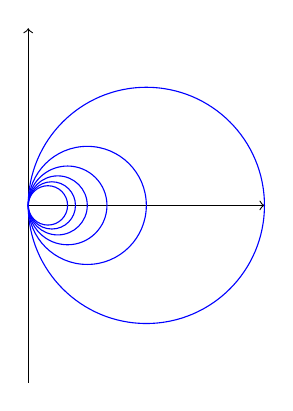
\begin{tikzpicture}[scale=1.5]
        %\draw[help lines] (0,-3) grid (3,3);

        \draw[->] (0,-1.5) -- (0,1.5);
        \draw[->] (0,0) -- (2,0); 
        \foreach \n in {1,...,6}
            \draw[blue] (1/\n,0) circle (1/\n);
    \end{tikzpicture}
    \caption{Two examples of sets which are rectifiable, but not manifolds.}
\end{figure}

Having shown that $\scrH^k \restrict T_p M$ is a tangent measure to $\scrH^k \restrict M$ for any $k$-dimensional Lipschitz submanifold $M \subseteq \bbR^d$ and $\scrH^k$-a.e. $p \in M$, we now ask when is the opposite true? Namely, can we judge that a set is a submanifold by showing it has approximate tangent spaces a.e., where an \textit{approximate tangent space} to a set $S \subseteq \bbR^d$ at $p \in S$ is a $k$-dimensional vector space $V \subseteq \bbR^d$ such that $\scrH^k \restrict V \in \Tan(\scrH^k \restrict S,p)$. Immediately, we see this is not true at all, as illustrated by figure \ref{fig:rectifiable}. First, the union of the $x$-axis and the parabola $y = x^2$ in $\bbR^2$ has an approximate tangent space at every point, but it fails to be a manifold near the origin.

More absurdly, take $H$ to be the union of circles centered at $(\frac{1}{n},0)$ with radius $\frac{1}{n}$ in $\bbR^2$ ($n \in \mathbb{N}$), the so-called \textit{Hawaiian earring}. The fundamental group $\pi_1(H)$ is famously complicated. In particular, it is uncountable, and therefore cannot be a topological manifold (see [Lee, Topological Manifolds, thm 7.21]). Despite this, it has approximate tangent spaces at a.e. point. Although since it exhibits some self-similarity at the origin, it is actually true that $\scrH^1 \restrict H$ is a tangent measure to itself at 0.

The thread linking our two counterexamples is that they are countable unions of submanifolds of $\bbR^d$, and this will turn out to be the correct generalization. We say a $\mathscr{H}^k$-measurable subset $E \subseteq \bbR^d$ is called $k$-\textit{rectifiable} if there exist Lipschitz maps $f_i \colon \bbR^k \to \bbR^d$, $i = 1,\dots,\infty$, such that 
\begin{equation}
    \mathscr{H}^k\left(E \setminus \bigcup_{i=1}^\infty f_i(\bbR^k)\right) = 0
\end{equation}
Rectifiable sets are in abundance. For a Borel set in $\bbR^d$ with locally finite perimeter, its measure-theoretic boundary turns out to be rectifiable. See \textbf{[Krantz \& Parks, Geometry of Domains in Space, §3.7]} for more information.

As a technical aside to state the next theorem, we need to quickly introduce Hausdorff densities. Fix a Radon measure $\mu \in \scrM(\bbR^d)$, a point $p \in \bbR^d$, and $s > 0$. Define the \textit{upper Hausdorff} $s$-\textit{density} of $\mu$ at $p$ to be
\begin{equation}
    \Theta^{s*}(\mu,p) := \limsup_{r \downarrow 0} \frac{\mu(B(p,r))}{r^s},
\end{equation}
and the \textit{lower Hausdorff} $s$-\textit{density} to be
\begin{equation}
    \Theta^s_*(\mu,p) := \liminf_{r \downarrow 0} \frac{\mu(B(p,r))}{r^s}.
\end{equation}
If both densities agree, we write $\Theta^s(\mu,p)$ for their common value, and call it the \textit{Hausdorff} $s$-\textit{density}.

The following theorem classifies the tangents of rectifiable sets.
\begin{theorem}\label{thm:rectifiableFlatSets}
    Fix $k \in \bbN$, and let $E \subseteq \bbR^d$ be $\mathscr{H}^k$-measurable with finite $\mathscr{H}^k$-measure, and such that $\Theta_*^k(E,p) > 0$ for $\mathscr{H}^k$-a.e. $p \in E$. Then $E$ is $k$-rectifiable if and only if for $\mathscr{H}^k$-a.e. $p \in E$, there exists an $k$-dimensional vector subspace $V_p \subseteq \bbR^d$ such that $\Tan(\mathscr{H}^k \vert_E,p) = \set{ c \scrH^k \restrict V_p : c > 0 }$.
\end{theorem}
As with most other things in geometric measure theory, the proof of theorem \ref{thm:rectifiableFlatSets} is highly technical, involving study of the truncated ``light cone"-shaped set
\begin{equation}
    E \cap B(p,r) \cap \{ x \in \bbR^d : d(x-p,V) < s\left|x-p\right| \},
\end{equation}
where $r,s > 0$ and $V$ is a $k$-dimensional subspace of $\bbR^d$ (figure \ref{fig:cone}). See \textbf{[Mattila §§15-16]} for more details.

\begin{figure}
    \centering
    \begin{tikzpicture}
        %\draw[gray] (0,0) grid (10,5);

        \draw (1,1) -- (9,4);
        %\draw (8,5) -- ++(0.9,-2.4);
        \node[right] (V) at (9,4) {$V$};
        \draw[red] (2,0) -- (8,5);
        \draw[red] (5-3.9,2.4) -- (8+0.9,5-2.4);
        \node[above] (p) at (5,2.5) {$p$};
        \filldraw[red] (5,2.5) circle (0.05);
        \draw[blue] (5,2.5) circle (1.5);
    \end{tikzpicture}
    \caption{Truncated ``light cone'' around a point $p$}
    \label{fig:cone}
\end{figure}

More generally, a Radon measure $\mu \in \scrM(\bbR^d)$ is said to be $k$-\textit{rectifiable} if $\mu$ is absolutely continuous with respect to $\mathscr{H}^k$, and there exists a $k$-rectifiable Borel set $E \subseteq \bbR^d$ such that $\mu(\bbR^d \setminus E) = 0$. We can generalize theorem \ref{thm:rectifiableFlatSets} to measures in the following way:
\begin{theorem} \label{thm:rectifiableFlatMeasures}
    Fix $k \in \bbN$, and let $\mu \in \scrM(\bbR^d)$ be a Radon measure such that $0 < \Theta_*^k(\mu,p) \leq \Theta^{k*}(\mu,p) < \infty$ for $\mu$-a.e. $p \in \bbR^d$. Then $\mu$ is $k$-rectifiable if and only if for $\scrH^k$-a.e. $p \in \bbR^d$, there exists a $k$-dimensional vector subspace $V_p \subseteq \bbR^d$ such that $\Tan(\mu,p) = \set{ c \scrH^k \restrict V_p : c > 0 }$.
\end{theorem}
The additional condition on the upper Hausdorff density of $\mu$ is vital (at least for $d=1$), as we will see with the Preiss measure later.

A Radon measure $\mu \in \scrM(\bbR^d)$ on is called $k$-\textit{flat} if there exists a $k$-dimensional vector subspace $V \subseteq \bbR^d$ and $c \in (0,\infty)$ such that $\mu = c \mathscr{H}^k \restrict V$. In the case of the above Hausdorff density condition, Rectifiable measures are therefore the ``upper bound'' on measures with flat tangent measures.

\section{Measures with Multiple Tangent Measures}
\subsection{Measures with Stranger Tangent Measures}

In the previous chapter on rectifiability, we saw examples of measures whose tangent measures are well-behaved. In particular, all tangent measures $\tau$ we saw satisfied (at least almost everywhere)
\begin{equation}
    \tau(B(p,r)) = r^\alpha \tau(B(p,1))
\end{equation}
for some $\alpha > 0$. Such measures are called $\alpha$-\textit{uniform}. In this chapter, we will demonstrate that this property is not uniform (haha) among all tangent measures. First, for any arbitrary measure $\tau$ and a point $p \in \bbR^d$, we will define a measure $\mu$ which has $\tau$ as a tangent measure at $p$.

Fix $\tau \in \scrM(\bbR^d)$ and $p \in \bbR^d$. We will show there exists $\mu \in \scrM(\bbR^d)$ with $\tau \in \Tan(\mu,p)$. Fix $\epsilon \in (0,1)$, set $s_1 := 1$, and inductively define $s_j := \epsilon^j s_{j-1}$. Define $\mu \in \scrM(\bbR^d)$ by
\begin{equation}
    \int_{\bbR^d} \phi \; \d\mu := \int_{\bbR^d} \phi\parens{ \sum_{i=1}^\infty x s_i } \; \d\tau(x) \quad \text{for all } \phi \in C_c(\bbR^d).
\end{equation}
We then have 
\begin{equation}
    \int_{\bbR^d} \phi \; \d\mu_{p,s_j} = \int_{\bbR^d} \phi\parens{ \sum_{i=1}^\infty (x - p)\frac{s_i}{s_j} } \; \d\tau.
\end{equation}
The terms in the sum with $j > i$ become arbitrary large (on the order of at least $\epsilon^{-j}$) as $j \to \infty$. Similarly, the terms in the sum with $j < i$ become arbitrarily small (on the order of at most $\epsilon^{j+1}$ as $j \to \infty$. By continuity and compact support of $\phi$, we may take $j \to \infty$ to see that this converges to
\begin{equation}
    \int_{\bbR^d} \phi \; \d\tau.
\end{equation}
Therefore $\tau$ is a tangent measure to $\mu$ at $p$. 

\subsection{The O'Neil Measure}
All measures we have constructed so far have had unique tangent measures up to multiplication. Do there exist measures $\mu$ such that $\Tan(\mu,p)$ contains distinct tangent measures for some point $p \in \bbR^d$? There certainly are - example 14.2(3) in \textbf{[Mattila]} is one. In this section, we will construct a measure $\mu$ such that $\Tan(\mu,p)$ at $\mu$-a.e. point $p \in \bbR^d$ is all of $\scrM(\bbR^d)$. Naturally, this is the worst it can possibly be, although we will see later on that this is not actually uncommon for Radon measures. 

The following theorem was introduced by Toby O'Neil in \textbf{[O'Neil]}, and the proof will follow his method.
\begin{theorem}[O'Neil] \label{thm:oneil}
    Fix $d \in \bbN$. There exists a Radon measure $\mu \in \scrM(\bbR^d)$ such that for $\mu$-a.e. $p \in \bbR^d$, we have $\Tan(\mu,p)$.
\end{theorem}
\begin{proof}
    Define the set $\scrS \subseteq \scrM(\bbR^d)$ to be the set of convex linear combinations of Dirac measures $\delta_x$ for $x \in \bbQ^d \cap B(0,1)$, with $\delta_0$ always included in the convex linear combination. That is,
    \begin{equation} \label{eq:setOfMeasuresForOneilMeasure}
        \scrS := \left\{ \alpha_0 \delta_0 + \sum_{i=1}^N \alpha_i \delta_{x_i} \;\middle|\;
        \begin{aligned} 
            &N \in \bbN, \alpha_i \in \bbQ \cap (0,1), \sum_{i=0}^N \alpha_i = 1, \\
            &x_i \in \bbQ^d \cap B(0,1), x_i \neq x_j \text{ for } i \neq j 
        \end{aligned}
        \right\}.
    \end{equation}
    We show that the set $\{ p\nu_{0,q} : p,q \in \bbQ^+, \nu \in \scrS \}$ is weakly* dense in $\scrM(\bbR^d)$. First, note that the set of measures with compact support in $\scrM(\bbR^d)$ is dense in $\scrM(\bbR^d)$. This can be shown, for example, by considering the compactly supported measures $\mu \restrict B(0,N)$ for $N \in \bbN$. 
    Fix, therefore, a compactly supported $\mu \in \scrM(\bbR^d)$. Given $m \in \bbN$, let $\scrQ_m$ be the family of half-open cubes in $\bbR^d$ with side length $\frac{1}{m}$ congruent to $Q_0 = [-\frac{1}{2m},\frac{1}{2m})$. Let $x_Q$ be the midpoint of $Q \in \scrQ_m$. Certainly, we have that
    \begin{equation} \label{eq:riemsum}
        \begin{aligned}
            \abs{ \int_{\bbR^d} f \, \d{\mu} - \sum_{Q \in \scrQ_m} f(x_Q)\mu(Q) } 
            &= \abs{ \int_{\bbR^d} f - \sum_{Q \in \scrQ_m} f(x_Q) \mathbbm{1}_Q \, \d{\mu} } \\
            &\leq \int_{\bbR^d} \sum_{Q \in \scrQ_m} \abs{ f(x) - f(x_Q) } \mathbbm{1}_Q(x) \, \d{\mu(x)} \\
            &\leq \int_{\bbR^d} \sum_{Q \in \scrQ_m} \abs{x-x_Q} \mathbbm{1}_Q(x) \, \d{\mu(x)} \\
            &\rightarrow 0 \text{ as } m \to \infty
        \end{aligned}
    \end{equation}
    for all Lipschitz $f$ with compact support and with Lipschitz constant at most 1. The latter integral converges to 0 by the dominated convergence theorem, since $\mu$ has compact support.
    Fix $\epsilon > 0$, and choose $m_0 \in \bbN$ such that $m \geq m_0$ implies 
    \begin{equation} \label{m0definition}
        \abs{ \int_{\bbR^d} f \, \d{\mu} - \sum_{Q \in \scrQ_m} f(x_Q)\mu(Q) } < \epsilon
    \end{equation}
    for all $f \in \Lip_{\leq 1}(\bbR^d)$. Such a choice is possible by \eqref{eq:riemsum}.
    Since $\mu$ has compact support, there exists $N \in \bbN$ such that $\mu(Q) = 0$ whenever $Q \cap B(0,N) = \emptyset$, so that 
    \begin{equation} 
        \sum_{Q \in \scrQ_m} f(x_Q)\mu(Q) = \sum_{\substack{Q \in \scrQ_m \\ Q \cap B(0,N) \neq \emptyset}} f(x_Q)\mu(Q)
    \end{equation}
    Write $\widetilde{\scrQ}_m = \{ Q \in \scrQ_m : Q \cap B(0,N) \neq \emptyset \}$.
    Next, index the elements $Q_i$ of $\scrQ_m$ by $i \in \bbN \cup \{0\}$, with $Q_0$ being the cube centered at 0 as above. For each $i \in \bbN \cup \{0\}$, let $p_{Q_i} \in \bbQ^+$ be such that $\abs{ \mu(Q_i) - p_{Q_i} } < \frac{\epsilon}{2^{i+1}}$. In particular, if $Q_i \notin \widetilde{\scrQ}_m$, we can set $p_{Q_i} = 0$. We must, however, have that $p_{Q_0} > 0$. Similarly, for each $i \in \bbN \cup \{0\}$, let $x_{Q_i}^* \in \bbQ^n$ be such that $\abs{ x_{Q_i} - x_{Q_i}^* } < \frac{\epsilon}{2^{(i+1)} p_{Q_i} }$. We then have
    \begin{equation}
        \begin{aligned}
            \abs{ \sum_{Q \in \scrQ_m} f(x_Q)\mu(Q) - \sum_{Q \in \scrQ_m} f(x_Q^*)p_Q }
            &\leq \abs{ \sum_{Q \in \scrQ_m} f(x_Q)\mu(Q) - \sum_{Q \in \scrQ_m} f(x_Q)p_Q }\\
            &\hspace{20pt} + \abs{ \sum_{Q \in \scrQ_m} f(x_Q)p_Q - \sum_{Q \in \scrQ_m} f(x_Q^*)p_Q } \\
            &\leq \sum_{Q \in \scrQ_m} f(x_Q) \abs{ \mu(Q) - p_Q }
                + \sum_{Q \in \scrQ_m} \abs{ f(x_Q) - f(x_Q^*) }p_Q \\
            &\leq \norm{f}_\infty \sum_{i=0}^\infty \frac{\epsilon}{2^{i+1}}
                + \sum_{Q \in \scrQ_m} \abs{ x_Q - x_Q^* }p_Q \\
            &\leq \norm{f}_\infty \epsilon + \sum_{i=0}^\infty \frac{\epsilon}{2^{i+1} p_{Q_i}} p_{Q_i} \\
            &= \epsilon(1 + \norm{f}_\infty).
            \end{aligned}
    \end{equation}
    for all Lipschitz $f$ with compact support and with Lipschitz constant at most 1. 
    
    For each $Q \in \widetilde{\scrQ}_m$, set $y_Q^* := \frac{x_Q^*}{N+1} \in \bbQ^n \cap B(0,1)$. Then 
    \begin{equation}
        \begin{aligned}
            \sum_{Q \in \widetilde{\scrQ}_m} p_Q \delta_{x_Q^*} 
            &= \sum_{Q \in \widetilde{\scrQ}_m} p_Q \delta_{Ny_Q^*} \\
            &= \left( \sum_{Q \in \widetilde{\scrQ}_m} p_Q \delta_{y_Q^*} \right)_{0,N^{-1}} \\
            &= \left( \sum_{Q \in \widetilde{\scrQ}_m} p_Q \right) \left( \sum_{Q \in \widetilde{\scrQ}_m} \frac{p_Q}{\sum_{Q \in \widetilde{\scrQ}_m} p_Q} \delta_{y_Q^*} \right)_{0,N^{-1}} \\
            &=: p \nu_{0,N^{-1}}.
        \end{aligned}
    \end{equation}
    Let $f \in \Lip_{\leq 1}(\bbR^d)$. By our calculations above, we have that for $m \geq m_0$ (where $m_0$ was defined in \eqref{m0definition}),
    \begin{equation}
        \begin{aligned}
          \abs{ \int_{\bbR^d} f \, \d{\mu} - \int_{\bbR^d} f \, \d{(p\nu_{0,N^{-1}})} }
          &= \abs{ \int_{\bbR^d} f \, \d{\mu} - \sum_{Q \in \widetilde{\scrQ}_m} f(x_Q^*) p_Q } \\
          &= \abs{ \int_{\bbR^d} f \, \d{\mu} - \sum_{Q \in \scrQ_m} f(x_Q^*) p_Q } \\
          &\leq \abs{ \int_{\bbR^d} f \, \d{\mu} - \sum_{Q \in \scrQ_m} f(x_Q)\mu(Q) } \\
          &\hspace{20pt} + \abs{ \sum_{Q \in \scrQ_m} f(x_Q)\mu(Q) - \sum_{Q \in \scrQ_m} f(x_Q^*)p_Q } \\
          &\leq \epsilon + \epsilon(1 + \norm{f}_\infty) \\
          &= \epsilon(2 + \norm{f}_\infty).
        \end{aligned}
    \end{equation}
    By construction, $\nu$ is an element of $\scrS$. Since $\epsilon > 0$ was arbitrary, we are done.

    Because of this and lemma \ref{lem:tangent_measure_properties}, it suffices to find a measure $\mu$ such that $\scrS \subseteq \Tan(\mu,p)$ for $\mu$-a.e. $p \in \bbR^d$. Indeed, lemma \ref{lem:tangent_measure_properties} parts (a) and (b) mean the set $\{ c\nu_{0,r} : c,r>0 \}$ is contained in $\Tan(\mu,p)$, and by the above analysis, this means $\Tan(\mu,p)$ is dense in $\scrM(\bbR^d)$. By part (c) of lemma \ref{lem:tangent_measure_properties}, we infer that $\Tan(\mu,p)$ is all of $\scrM(\bbR^d)$ for $\mu$-a.e. $p \in \bbR^d$. 

    Note that $\scrS$ is a countable set. Index the elements $\widetilde{\nu}_i$ of $\scrS$ by $i \in \bbN$.
    Define the sequence $(i_k)_{k \in \bbN \cup \{0\}}$ by 
    \begin{equation}
        \begin{aligned}
            i_0 &= 0; \\
            i_k &= k - \frac{1}{2}n(n+1) \text{ for } k \in \left[ \frac{1}{2}n(n+1), \frac{1}{2}(n+1)(n+2) \right), n \in \bbN.
        \end{aligned}
    \end{equation}
    That is, $i_k$ is the sequence $(1,1,2,1,2,3,1,2,3,4,\dots)$. If $k_n = \frac{1}{2}n(n+1)$ for $n \in \bbN \cup \{0\}$, then $i_{k_n} = 1$. More generally for $m \in \bbN$, define
    \begin{equation}
        k_m(n) = \frac{1}{2}(n+m-1)(n+m) + (m-1) \text{ for } n \geq 0.
    \end{equation}
    Then $k_m(n) = m$ for $n \geq 0$. We set $\nu_k := \widetilde{\nu}_{i_k}$. It follows that every element of $\scrS$ occurs infinitely many times in the sequence $(\nu_k)$. In particular, $\nu_{k_m(n)} = \widetilde{\nu}_m$ for all $n \geq m-1$.

    For each $k \in \bbN$, we write 
    \begin{equation}
        \nu_k = \alpha_k(0) \delta_0 + \sum_{j = 1}^{N_k} \alpha_k(x_{k,j}) \delta_{x_{k,j}}.
    \end{equation}
    For each $k \in \bbN$, define $\Omega_k := \{0,x_{k,1},\dots,x_{k,N_k}\}$. Each $\alpha_k$ can be interpreted as the probability mass function for the measure $\nu_k$ on $(\Omega_k, 2^{\Omega_k})$. We then set $\Omega := \prod_{k=1}^\infty \Omega_k$. Consider the $\sigma$-algebra $\scrA$ on $\Omega$ generated by the \textit{cylinder sets} of the form $\eta \vert_j = \{(\eta_1,\dots,\eta_j)\} \times \prod_{k=j+1}^\infty \{ x_{k,1},\dots,x_{k,N_k} \}$ for $\eta \in \Omega$, and define a probability measure $\alpha$ on $(\Omega, \scrA)$ by 
    \begin{equation}
        \alpha(\eta \vert_j) := \prod_{k=1}^j \alpha_k(\eta_k).
    \end{equation}
    That is, $(\Omega, \scrA, \alpha)$ is the product space $\prod_{k=1}^\infty (\Omega_k, 2^{\Omega_k}, \alpha_k)$.

    \begin{figure} 
        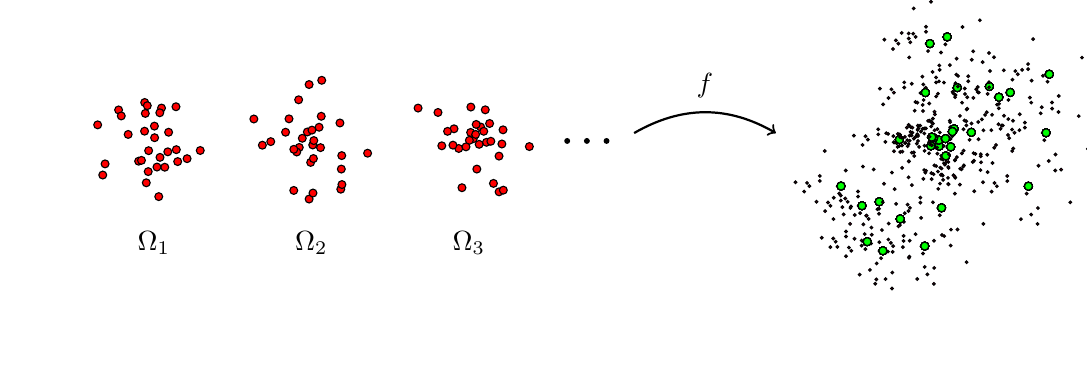
\begin{tikzpicture}
            %\draw[help lines] (0,0) grid (13,4);

            \foreach \j in {1,...,3}
            {
                \node at (2*\j - 1,.7) {$\Omega_\j$};
                \foreach \i in {1,...,30}
                {
                    \pgfmathsetmacro\radius{.8*rnd}
                    \draw[fill=red] (2*\j - 1,2) ++ (rnd*360:\radius) circle(0.05);
                }
            }
            \foreach \i in {1,2,3}
            {
                \draw[fill] (6,2) ++ (\i / 4,0) circle (0.03);
            }
            \draw[->,thick] (7,2) ++ (.1,.1) to [out=30, in=150] (8.9,2.1);
            \node at (8,2.7) {$f$};

            \coordinate (thebigone) at (11,2);
            \newsavebox{\cloud}
            \savebox{\cloud}
            {
                \foreach \i in {1,...,15}
                { 
                    \pgfmathsetmacro\radius{.6*rnd}
                    \draw[fill=green] (0,0) circle (0.05);
                    \draw[fill=purple] (rnd*360:\radius) circle(0.05*1/3);
                }
            }
            \foreach \i in {1,...,30}
            {
                \pgfmathsetmacro\radius{1.8*rnd}
                \draw[fill=purple] (thebigone) ++ (rnd*360:\radius) node {\usebox{\cloud}};
            }
 
        \end{tikzpicture}
        \caption{Mapping the product space $(\Omega,\scrA,\alpha)$ into $B(0,1)$.}
        \label{fig:oneilPushforwardMap}
    \end{figure}
     
    For each $k \in \bbN$, define 
    \begin{equation}
        \sigma_k := \min\set{ \abs{x - y} : x,y \in \Omega_k, x \neq y }.
    \end{equation}
    Inductively define the sequence $r_k$ by choosing $r_0 > 1$, and defining $r_k := \frac{r_0^{k}}{\sigma_k} r_{k-1}$.
    Define $f \colon \Omega \to B(0,1)$ by
    \begin{equation}
        f(\eta) := \sum_{k=1}^\infty \frac{\eta_k}{r_k}
    \end{equation}
    See figure \ref{fig:oneilPushforwardMap}. We set $\mu := f_* \alpha$ to be the pushforward measure of $\alpha$ by $f$ on the space $(\bbR^d, \scrB(\bbR^d))$. Our aim is to choose the $r_k$ so that as we zoom in to $\mu$-a.e. point in $B(0,1)$, we go through the sequence $\Omega_k$. In particular, we'd like the sequences $k_m$ to provide us with the different rates of zooming in.

    Given $m \in \bbN$, define
    \begin{equation}
        V_m := \{ \eta \in \Omega : \eta_{k_m(n)} = 0 \text{ i.o. in } n \}.
    \end{equation}
    That is, $V_m$ is the event of choosing the point $0$ infinitely often whenever $\nu_k = \widetilde{\nu}_m$.
    Now, since $\alpha(\eta_{k_m(n)} = 0) = \alpha_{k_m(n)}(0)$ is positive and constant with varying $n$, we have that 
    \begin{equation}
        \sum_{n=0}^\infty \alpha(\eta_{k_m(n)} = 0) = \infty.
    \end{equation}
    Since the events $\{ \eta_{k_m(n)} = 0 \}$ are independent, we conclude by the Borel-Cantelli lemma that $\alpha(V_m) = 1$. In other words, $\mu(f(V_m)) = 1$. Define $V = \bigcap_{m \in \bbN} V_m$ to be the event of selecting $0$ infinitely often along the whole sequence. By countability, $\alpha(V) = 1$.

    We will show that $\scrS \subseteq \Tan(\mu,p)$ for all $p \in f(V)$. Fix $p \in f(V)$, and write $p = f(\pi) = \sum_{k=1}^\infty \frac{\pi}{r_k}$ for some $\pi \in V$. Fix $m \in \bbN$, and let $n_j \in \bbN$ be a sequence with $n_j \rightarrow \infty$, and with $\pi_{k_m(n_j)} = 0$ for all $j$. This is possible by definition of $V$. Fix $\phi \in \Lip_{\leq 1}(\bbR^d)$. The proof will be concluded by lemma \ref{lem:equivalentDefinitionOfWeak*Convergence} once we show $\int_{\bbR^d} c_j \phi \; \d\mu_{\overline{x},s_j} \rightarrow \int_{\bbR^d} \phi \; \d\nu_m$ for some appropriate choice of $c_j$ and $s_j$. 
    
    Define the set $\Omega^{(j)} := \set{ \eta \in \Omega : \eta_k = \pi_k \text{ for } k = 1,\dots,k_m(n_j)-1 }$, and let $c_j = \alpha(\Omega^{(j)})^{-1}$. Also let $s_j = 1/r_{k_m(n_j)}$. We have
    \begin{equation}
        \int_{\bbR^d} \phi \; \d(c_j\mu_{\overline{x},s_j}) = c_j \int_{\bbR^d} \phi\parens{\frac{x - \overline{x}}{s_j}} \; \d\mu(x)
                                                            = c_j \int_{\Omega} \phi\parens{r_{k_m(n_j)} \sum_{k=1}^\infty \frac{\eta_k - \pi_k}{r_k}} \; \d\alpha(\eta).
    \end{equation}
    We also have 
    \begin{equation}
        \int_{\bbR^d} \phi \; \d\nu_m = \int_{\Omega_{k_m(n_j)}} \phi \; \d\nu_m = \int_\Omega \phi(\eta_{k_m(n_j)}) \; \d\alpha(\eta) 
        = c_j \int_{\Omega^{(j)}} \phi(\eta_{k_m(n_j)}) \; \d\alpha(\eta),
    \end{equation}
    where the last equality comes from the fact that the functions (random variables in this context) $\bbone_{\Omega^{(j)}}$ and $\eta \mapsto \phi(\eta_{k_m(n_j)})$ are independent.

    We would like to show, at least for $j$ large enough, that
    \begin{equation} \label{eq:restrictingAnIntegral}
        \int_{\Omega} \phi\parens{r_{k_m(n_j)} \sum_{k=1}^\infty \frac{\eta_k - \pi_k}{r_k}} \; \d\alpha(\eta) 
        = \int_{\Omega^{(j)}} \phi\parens{r_{k_m(n_j)} \sum_{k=1}^\infty \frac{\eta_k - \pi_k}{r_k}} \; \d\alpha(\eta),
    \end{equation}
    where $\Omega^{(j)} := \set{ \eta \in \Omega : \eta_k = \pi_k \text{ for } k = 1,\dots,k_m(n_j)-1 }$. Indeed, suppose this were true, and let $\eta$ be in this set. Then
    \begin{equation}
        \abs{ \eta_{k_m(n_j)} - r_{k_m(n_j)} \sum_{k=1}^\infty \frac{\eta_k - \pi_k}{r_k} } \leq  \sum_{k=k_m(n_j)+1}^\infty \frac{\abs{\eta_k - \pi_k}}{r_k}
        \leq \sum_{k=k_m(n_j)}^\infty \frac{1}{r_k},
    \end{equation}
    since all $\eta_k$ and $\pi_k$ are contained in $B(0,1)$, and $\pi_{k_m(n_j)} = 0$ by assumption. Since $\phi$ is Lipschitz with constant at most 1, this estimate implies
    \begin{equation} \begin{aligned}
        &\abs{ \int_{\bbR^d} \phi \; \d(c_j \mu_{\overline{x},s_j}) - \int_{\bbR^d} \phi \; \d\nu_m } \\
        &\quad = \abs{ c_j \int_{\Omega^{(j)}} \phi\parens{r_{k_m(n_j)} \sum_{k=1}^\infty \frac{\eta_k - \pi_k}{r_k}} \; \d\alpha(\eta)
                      - c_j \int_{\Omega^{(j)}} \phi(\eta_{k_m(n_j)}) \; \d\alpha(\eta) } \\
        &\quad \leq c_j \int_{\Omega^{(j)}} \sum_{k=k_m(n_j)} \frac{1}{r_k} \; \d\alpha \\
        &\quad = \sum_{k = k_m(n_j)}^\infty \frac{1}{r_k} \\
        &\quad \rightarrow 0,
    \end{aligned} \end{equation}
    noting that $\sum_{k=1}^\infty \frac{1}{r_k}$ certainly converges since $r_k$ increases very quickly.

    It remains to check (\ref{eq:restrictingAnIntegral}). Suppose $\eta \in \Omega \setminus \Omega^{(j)}$, and let $K < k_m(n_j)$ be the smallest integer with $\eta_K \neq \pi_K$. Let $R > 0$ be such that $\supp{\phi} \subseteq B(0,R)$. We have {\color{red} finish this. in particular, choose appropriate $r_k$}
\end{proof}

\subsection{Extensions and Conclusion}
Note that definition (\ref{eq:setOfMeasuresForOneilMeasure}) of the set $\scrS$ grants us some leeway in choosing $\mu$. Indeed, rather than taking $x_i \in \bbQ^d \cap B(0,1)$, we could ask that they come from a dense subset of another open ball, and the same proof would carry on over verbatim. One might wonder how restrictive the condition $\Tan(\mu,x_0) = \scrM(\bbR^d)$ actually is. All our examples in section 1 certainly didn't satisfy this, and it even took us a lot of work to show the existence of even one of these measures. As it turns out, this is not so restrictive at all. Tuomas Sahlsten in [Tangent Measures of Typical Measures,Tuomas Sahlsten,Real Analysis Exchange,Vol. 40, No. 1 (2014-2015), pp. 53-80] and Toby O'Neil in [A local version of the Projection Theorem and other results in Geometric Measure Theory,
PhD Thesis, University College London, 1994] independently managed to prove the following:
\begin{theorem} \label{thm:sahlstenTypicalMeasures}
    For a typical $\mu \in \scrM(\bbR^d)$, we have $\Tan(\mu,x_0) = \scrM(\bbR^d)$.
\end{theorem}
Here, \textit{typical} means this result holds for all $\mu$ in a residual subset (a countable union of dense open sets) of $\scrM(\bbR^d)$. The proof of theorem \ref{thm:sahlstenTypicalMeasures} is effectively a much more technical version of the construction above, making use of a set $\scrS$ similar to the above, and also explicitly defining the residual subset $\scrR \subseteq \scrM(\bbR^d)$.

{\color{red} hey billy can you use zorn's lemma to prove the o'neil theorem? i.e. say $\mu \prec \nu$ if there exists $N \subseteq \bbR^d$ with $\mu(N) = \nu(N) = 0$ and $\Tan(\mu,p) \subseteq \Tan(\nu,p)$ for all $p \in \bbR^d \setminus N$ then blah blah upper bound blah blah maximal element}

\section{Tangent Measures of Singular Measures}
\subsection{Tangent Measures of Pushforward Measures} \label{sec:pushforward}
Let $\mu \in \scrM(\bbR^m)$, and let $f \colon \bbR^m \to \bbR^d$ be a $C^1$ diffeomorphism. We would like to investigate the tangent measures of the pushforward measure $f_*\mu$. This investigation will follow many of the same lines as in section \ref{sec:submanifolds} Choose a tangent measure $\tau \in \Tan(\mu,q)$, and let $c_j \mu_{q,r_j}$ be a blowup sequence for $\tau$. By translating if necessary, we may assume $f(q) = 0$. Fix $\phi \in C_c(\bbR^d)$, and let $R > 0$ be such that $\supp{\phi} \subseteq B(0,R)$. Consider now 
\begin{equation} \begin{aligned}
    c_j \int_{\bbR^d} \phi \; \d(f_*\mu)_{0,r_j} &= c_j \int_{\bbR^d} \phi\parens{\frac{x}{r_j}} \; \d(f_* \mu)(x) \\
                                               &= c_j \int_{\bbR^m} \phi\parens{\frac{f(y)}{r_j}} \; \d\mu(y).
\end{aligned} \end{equation}
Note that since $f$ is a diffeomorphism, the set $f^{-1}(B(0,R))$ is bounded, so $f$ is uniformly Lipschitz on this set. Let $\Lip{f}$ be its Lipschitz constant on this set. If $y \in \bbR^m$ lies outside the set $B(0,rR/\Lip{f})$, then $f(y)/r$ lies outside the set $B(0,R)$ (again, cf. section \ref{sec:submanifolds}). So for $K := R/\Lip{f}$, the above integral is 
\begin{equation}
    c_j \int_{B(0,Kr_j)} \phi\parens{\frac{f(y)}{r_j}} \; \d\mu{y}.
\end{equation}
Now, we also have 
\begin{equation} \begin{aligned}
    &\lim_{j \to \infty} \abs{ c_j \int_{B(0,Kr_j)} \phi\parens{\frac{f(y)}{r_j}} \; \d\mu(y) - c_j \int_{B(0,Kr_j)} \phi\parens{\frac{\d f(0)(y)}{r_j}} \; \d\mu(y) } \\
    &\quad \leq \lim_{j \to \infty} c_j \mu(0,Kr_j) \, C \sup_{y \in B(0,Kr_j)} \frac{\abs{f(y) - \d f(0)(y)}}{r_j} \\
    &= 0,
\end{aligned} \end{equation}
where $C > 0$ is the Lipschitz constant of $\phi$. Here, we remark that by our study of the normalizing constants $c_j$ in section \ref{sec:blowingUp}, we may take $c_j = \mu(B(0,Kr_j))^{-1}$ without loss of generality, and the resulting tangent measure will be the same up to multiplication by a constant. This is of course inconsequential, since $\Tan(f_*\mu,0)$ is a cone by lemma \ref{lem:tangent_measure_properties}. Finally, we then have 
\begin{equation} \begin{aligned}
    \lim_{j \to \infty} c_j \int_{B(0,Kr_j)} \phi\parens{\frac{\d f(0)(y)}{r_j}} \; \d\mu(y) &= \lim_{j \to \infty} c_j \int_{\bbR^m} \phi\parens{\frac{\d f(0)(y)}{r_j}} \; \d\mu(y) \\
    &= \int_{\bbR^m} \phi\parens{ \d f(0)(y) } \; \d\tau(y) \\
    &= \int_{\bbR^d} \phi \; \d(\d f(0)_* \tau).
\end{aligned} \end{equation}
It follows that $\d f(0)_*\tau$ is a tangent measure to $f_*\mu$ at $0$.

\begin{figure} 
    \centering
    \begin{tikzpicture}
        %\draw[gray] (0,0) grid (15,6);

        \draw[blue] (1,3) -- (5,3);
        \draw[blue] (11.5,3) circle (1.5cm);
        \draw[->] (6,3) to[out=30,in=150] (9,3);
        \node (f) at (7.5,4) {$f$};
        \node (L) at (3,2) {$\scrL^1 \restrict [0,2\pi)$};
        \node (HS) at (11.5,1) {$\scrH^1 \restrict S^1$};
        \filldraw[red] (4,3) circle (0.05cm);
        \node (q) at (4,3.5) {$q$};
        \filldraw[red] (11.5-1.06,3+1.06) circle (0.05cm);
        \node (p) at (11.5-1.06+0.4,3+1.06-0.4) {$p$};
        \draw[red] (11.5-1.06-1.06,3+1.06-1.06) -- (11.5-1.06+1.06,3+1.06+1.06);
        \node[anchor=east] (HTpS) at (11,5) {$\scrH^1 \restrict T_pS^1 = \d f(q)_* \scrL^1$};
    \end{tikzpicture}
    \caption{Pushforward of Lebesgue measure}
    \label{fig:pushforwardLebesgue}
\end{figure}

Let's consider the example suggested by figure \ref{fig:pushforwardLebesgue}. Define the map $f \colon [0,2\pi) \subseteq \bbR \to \bbR^2$ by $f(s) := (\cos{s},\sin{s})$, whose image is a circle. Recall the area formula (\ref{eq:areaFormula}). Since the derivative of $f$ at $s$ is just the (column) vector $f'(s) = (-\sin{s},\cos{s})$, we may calculate its Jacobian determinant to be
\begin{equation}
    \mathrm{J}f(s) = \sqrt{f'(s)^\T f'(s)} = 1.
\end{equation}
Given $\phi \in C_c(\bbR^2)$, we use the area formula to calculate 
\begin{equation} \begin{aligned}
    \int_{\bbR^2} \phi \; \d(\scrH^1 \restrict S^1) &= \int_{S^1} \phi \; \scrH^1 \\
    &= \int_0^{2\pi} \phi(f(s)) \J f(s) \; \d\scrL^1(s) \\
    &= \int_0^{2\pi} \phi(f(s)) \; \d\scrL^1(s) \\
    &= \int_\bbR \phi \; \d(f_*(\scrL^1 \restrict [0,2\pi)).
\end{aligned} \end{equation}
It follows that $\scrH^1 \restrict S^1$ is the pushforward measure $f_*\scrL^1$. Now fix a point $p = f(q) \in S^1$. In section \ref{sec:submanifolds}, we calculated that a tangent measure of $\scrH^1 \restrict S^1$ at $p$ is $\scrH^1 \restrict T_p S^1$. Our above calculations for tangent measures of pushforward measure shows that $\d f(q)_* \scrL^1$ is a tangent measure to $f_* (\scrL^1 \restrict [0,2\pi))$ at $p$. However, we know that $\d f(q)$ is given by $f'(q) = (-\sin{q},\cos{q})$, so the image of $\d f(q)$ is precisely the tangent space $T_p S^1$. Using the area formula again, we see that our theory from this section and section \ref{sec:submanifolds} do not contradict each other.


\subsection{Hausdorff Density and Singularities}
Consider the measure $\mu = \delta_0 + \scrL^d$ on $\bbR^d$. Certainly, this measure is not singular with respect to $\scrL^d$ in the sense that its null sets are completely indistinct from those of Lebesgue measure, but there is certainly a problem at the origin. This invites us to consider defining a notion of ``singularity'' at a point in $\bbR^d$.

Recall the definition of Hausdorff density from section \ref{sec:rectifiability}. Immediately from the defition, we see $\Theta^d(\scrL^d,p) = \omega_d$ for all $p \in \bbR^d$, where $\omega_d$ is the volume of the unit ball in $\bbR^d$. Some authors put a constant in the denominator of the definition of the upper and lower Hausdorff densities to ensure $\Theta^d(\scrL^d,p) = 1$, but the exact value is not important, at least for our purposes. More generally, we have $\Theta^s(\scrH^s,p) = \omega_s$ for some $\omega_s > 0$. For our measure $\mu = \delta_0 + \scrL^d$ as above, it is easy to see that $\Theta^d(\mu,p) = \omega_d$ for $p \neq 0$, and $\Theta^d(\mu,0) = \infty$. 

Some simple properties of Hausdorff densities: {\color{red} do this}


Actually, David Preiss in {\bf [Preiss]} introduced tangent measures to prove the following long-standing conjecture {\color{red} was it long-standing?} in geometric measure theory:
\begin{theorem}[Marstrand]
    Let $\mu \in \scrM(\bbR^d)$ be a Radon measure. Suppose there exists $s > 0$ such that the Hausdorff density $\Theta^s(\mu,p)$ exists and is positive and finite for all $p$ in a set of positive $\mu$-measure. Then $s$ is an integer.
\end{theorem}
In fact, Preiss proved the following stronger theorem:
\begin{theorem}[Preiss] \label{thm:preissMarstrand}
    Let $\mu \in \scrM(\bbR^d)$ be a Radon measure, and $k \in \bbN$ a positive integer. If the Hausdorff density $\Theta^k(\mu,p)$ exists and is positive and finite for all $p$ in the support of $\mu$, then $\mu$ is $k$-rectifiable.
\end{theorem}
Theorem \ref{thm:rectifiableFlatMeasures} says that it suffices to show this condition on the Hausdorff density implies we have flat tangent measures at $\mu$-a.e. point. See {\bf [de Lellis]} for a more thorough outline of the proof, or {\bf [Mattila chapter 14]} for  a direct proof of Marstrand's theorem.


\subsection{The Preiss Measure}
Our interest is showing that a partial converse to theorem \ref{thm:preissMarstrand} for $d=1$ is not true: namely, we can find a measure $\mu$ which has flat tangent measures at $\mu$-a.e. point, but whose Hausdorff 1-density at $\mu$-a.e. point is infinite. Stated as a theorem:
\begin{theorem}[Preiss]
    There exists a Radon measure $\mu \in \scrM(\bbR)$ such that for $\mu$-a.e. $p \in \bbR$, we have $\Theta^{1*}(\mu,p) = \infty$, and $\Tan(\mu,p) = \set{c \scrL^1 : c > 0}$.
\end{theorem}
We will sketch a proof of this theorem here, details can be found in {\bf [Preiss 5.8]}.

As was the case with the O'Neil measure, the Preiss measure will be of the form $\mu = f_* \scrL \restrict (0,1)$ for some function $f \colon (0,1) \to \bbR$. To motivate the proof, let's determine what $f$ should look like. By our calculations in section \ref{sec:pushforward}, we would like any notion of gradient of $f$ to be somewhat constant. On the other hand, the singularity condition $\Theta^{1*}(\mu,p) = \infty$ means the Lebesgue measure of $f^{-1}(B(p,r))$ should be approximately $r^{1-\epsilon}$ for some small $\epsilon \in (0,1)$.

The construction employed is dyadic. We will construct a sequence of approximate gradients of $f$, and show their antiderivatives converge to the thing we're looking for. We will try to find $\mu$ directly satisfying the singularity condition 
\begin{equation}
    \Theta^{1\ast}(\mu,f(t)) = \limsup_{r \downarrow \infty} \frac{\mu(B(f(t),r))}{r} = \infty \quad \text{for } \scrL^1\text{-a.e. } t \in (0,1),
\end{equation}

and for $\scrL^1$-a.e. $t \in (0,1)$ and $\tau \in \Tan(\mu,f(t))$, we want to find $c > 0$ such that $\Theta^{1}(\tau,p) = c$ for all $p \in \bbR$. Indeed, this implies 
\begin{equation}
    \frac{\d\tau}{\d\scrL^1}(p) = c,
\end{equation}
for all $p \in \bbR$, so by the Besicovitch differentiation theorem (theorem \ref{thm:besicovitch}), we must have $\tau = c\scrL^1$.

Having discussed our motivation for the construction, let's begin the construction. This construction will be based on a collection of dyadic subintervals of $[0,1)$ of the form $[i2^{-k},(i+1)2^{-k})$. We will define them rigourously by induction. To start let $Q := [0,1)$. Next, given $Q_{i_1,\dots,i_{k-1}} \subseteq Q$ define $Q_{i_1,\dots,i_{k-1},0}$ to be the first half-open subinterval of $Q_{i_1,\dots,i_{k-1}}$ of size $2^{-k}$, and $Q_{i_1,\dots,i_{k-1},1}$ to be the second. The construction intervals $Q_i$ are therefore enumerated by binary sequences $i = (i_1,\dots,i_k) \in \set{0,1}^k$. The integer $k$ is called the \textit{generation} of the interval $Q_i$. The \textit{children} of $Q_i$ are $Q_{i0}$ and $Q_{i1}$, and $Q_i$ is the children's \textit{parent}. Given a binary sequence $i = (i_1,\dots,i_k)$, its \textit{parity} $\abs{i}$ is defined to be the sum $i_{k-1} + i_k$, with addition taken mod 2. For example, the parity of the sequence $011010$ is $1$, and the parity of $1010111$ is $1 + 1 = 0$. See figure \ref{fig:binaryIntervals}.

\begin{figure}
    \centering
    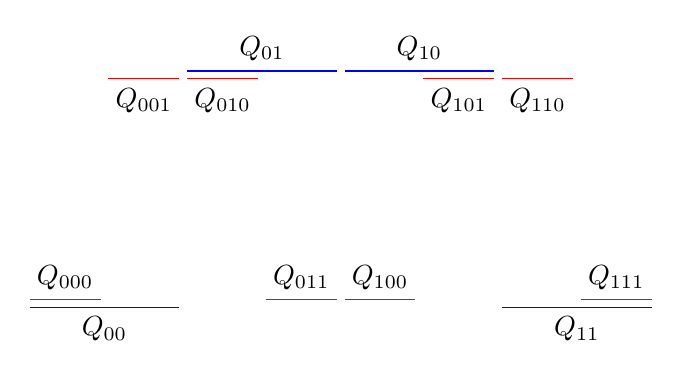
\begin{tikzpicture}
        %\draw[gray] (0,0) grid (10,5);

        \draw[blue] (0.05,0) -- (1.95,0) (2.05,3) -- (3.95,3) (4.05,3) -- (5.95,3) (6.05,0) -- (7.95,0);
        \draw[red] (0.05,0.1) -- (0.95,0.1) (1.05,2.9) -- (1.95,2.9) (2.05,2.9) -- (2.95,2.9) (3.05,0.1) -- (3.95,0.1) (4.05,0.1) -- (4.95,0.1) (5.05,2.9) -- (5.95,2.9) (6.05,2.9) -- (6.95,2.9) (7.05,0.1) -- (7.95,0.1);

        \draw node[above] at (0.5,0.1) {$Q_{000}$} node[below] at (1.5,2.9) {$Q_{001}$} node[below] at (2.5,2.9) {$Q_{010}$} node[above] at (3.5,0.1) {$Q_{011}$} node[above] at (4.5,0.1) {$Q_{100}$} node[below] at (5.5,2.9) {$Q_{101}$} node[below] at (6.5,2.9) {$Q_{110}$} node[above] at (7.5,0.1) {$Q_{111}$};

        \draw node[below] at (1,0) {$Q_{00}$} node[above] at (3,3) {$Q_{01}$} node[above] at (5,3) {$Q_{10}$} node[below] at (7,0) {$Q_{11}$};
    \end{tikzpicture}
    \caption{Construction intervals and corresponding parity}
    \label{fig:binaryIntervals}
\end{figure}

Having defined the construction intervals, we define the functions $g_k \colon Q \to \bbR$ inductively. In effect, $g_k$ is defined by a sequence of ``microadjustments''. Define $g_0 \colon Q \to \bbR$ by $g_0(t) = 1$ for all $t \in Q$, and fix $\epsilon_0 \in (0,1)$. Suppose $g_{k-1}$ and $\epsilon_{k-1}$ have been defined, and set 
\begin{equation}
    g_k(t) := \parens{1 + \sum_{i \in \set{0,1}^k} s_i \bbone_{Q_i}(t)} g_{k-1}(t),
\end{equation}
where $s_i = 0$ if $\abs{g_{k-1}(s)} < \epsilon_{k-1}$ for some (hence all) $s$ in the parent of $Q_i$, and $s_i = (-1)^{\abs{i}} \epsilon_{k-1}$ otherwise. We also let $\epsilon_k = \epsilon_{k-1}$ if 
\begin{equation} \begin{aligned}
    &\quad \abs{\set{t \in Q : \abs{g_{j-1}(t)} > \epsilon_{k-1} \text{ for } j = 0,\dots,k-1}} \geq \epsilon_{k-1} \\
    & \text{ or } \abs{\set{t \in Q : \abs{g_{k-1}(t)} \leq 1 \text{ for } j = 0,\dots,k-1}} \geq \epsilon_{k-1},
\end{aligned} \end{equation}
and $\epsilon_k = \epsilon_{k-1}/2$ otherwise. We also set 
\begin{equation}
    f_k(t) := \int_0^t g_k(s) \; \d s.
\end{equation}
See figure \ref{fig:iterationsOfG} for some iterations of $g$.

\begin{figure}
    \includegraphics[width=\textwidth]{Figure_3.png}
    %\includegraphics[width=0.5\textwidth]{iterationsOfGEpsilonLarge.png}
    
    \caption{Some iterations of $g_k$ for $\epsilon_0 = 0.1$.}
    \label{fig:iterationsOfG}
\end{figure}

Now, for all construction intervals $Q_i$ of generation $k$, we have $f_{k+1}(t) = f_k(t)$ whenever $s$ is one of the endpoints of $Q_i$ {\color{red} detailify this by using definition of $s_i$}. Fix $t \in Q$, and let $Q_i = [a,b)$ be the generation $k$ construction interval in which $t$ lies. Then 
\begin{equation} \begin{aligned}
    f_{k+1}(t) - f_k(t) &= \int_0^t g_{k+1}(s) - g_k(s) \; \d s \\
                        &= \int_a^t g_{k+1}(s) - g_k(s) \; \d s \\
                        &\leq \int_a^t \epsilon_k g_k(s) \; \d s \\
                        &= (t-a) \epsilon_k g_k(a) \\
                        &\leq 2^{-k} \epsilon_k (1 + \epsilon_0)^k,
\end{aligned} \end{equation}
since $g_k$ is constant on $[a,t)$. Taking suprema over $t \in [0,1]$, it follows that $\norm{f_{k+1} - f_k}_{L^\infty} \leq 2^{-k} \epsilon_0 (1 + \epsilon_0)^k$. Since $\sum_{k=1}^\infty \parens{\frac{1+\epsilon_0}{2}}^k < \infty$, the sequence $f_k$ is Cauchy in $C([0,1])$, so converges uniformly to some $f \in C([0,1])$. 

The aim now is to show $\mu := f_* \scrL^1 \restrict Q$ is the measure we want. This will follow by finding a function $h \colon Q \times (0,\infty) \to (0,\infty)$ such that for $\scrL^1$-a.e. $t \in Q$, we have
\begin{enumerate}[label=(\arabic*)] 
    \item \begin{equation} \label{eq:asymptoticEquiv}
        \lim_{r \downarrow 0} \frac{\mu(B(f(t),r))}{h(t,r)} = 1,
    \end{equation}

    \item \begin{equation} \label{eq:singular}
        \limsup_{r \downarrow 0} \frac{h(t,r)}{r} = \infty, \text{ and}
    \end{equation}

    \item \begin{equation} \label{eq:uniformity}
        \lim_{r \downarrow 0} \frac{h(t,sr)}{h(t,r)} = s \text{ for all } s > 0.
    \end{equation}
\end{enumerate}
Indeed, (1) and (2) immediately imply $\Theta^{1*}(\mu,f(t)) = \infty$. Meanwhile for $\tau \in \Tan(\mu,f(t))$ with $c\mu(B(f(t),r_j)^{-1} \mu_{f(t),r_j} \weakstar \tau$, we use lemma \ref{lem:semicontinuityOfWeak*Convergence}, (1), and (3) to calculate
\begin{equation} \begin{aligned}
    \Theta^1(\tau,0) &= \lim_{r \downarrow 0} \frac{\tau(B(0,r))}{r} \\
                     &\leq \lim_{r \downarrow 0} \liminf_{j \to \infty} \frac{c \mu_{f(t),r_j}(B(0,r))}{r\mu(B(f(t),r_j))} \\
                     &= \lim_{r \downarrow 0} \liminf_{j \to \infty} \frac{c}{r} \frac{ h(t,r_j) }{ \mu(B(f(t),r_j)) } \frac{ \mu(B(f(t),r_j r)) }{ h(t,r_j r) } \frac{ h(t,r_jr) }{ h(t,r_j) } \\
                     &= \lim_{r \downarrow 0} \frac{c}{r} r \\
                     &= c.
\end{aligned} \end{equation}
A similar calculation for $\tau(\overline{B(0,r)})$ is possible, which then shows $\Theta^1(\tau,0) = c$. To show $\Theta^1(\tau,p) = c$ for all other $p \in \bbR$, we {\color{red} do what? use continuity of $\mu$?}.

Let's now show such a function $h$ does exist. Immediately from the construction, we see
\begin{equation} \begin{aligned}
    g_k(t) &= \abs{1 + \sum_{i \in \set{0,1}^k} s_i \bbone_{Q_i}(t)} \abs{g_{k-1}(t)} \\
                 &\leq (1 + \epsilon_k) \abs{1 + \sum_{i \in \set{0,1}^{k-1}} s_i \bbone_{Q_i}(t)} \abs{g_{k-2}(t)} \\
                 &\leq \cdots \\
                 &\leq \prod_{j=1}^k (1 + \epsilon_k) \\
                 &\leq (1 + \epsilon_0)^k
\end{aligned} \end{equation}
for all $t \in Q$ and $k \in \bbN$, and $g_k(t) \geq (1 - \epsilon_0)^k$ similarly.

We would like to find a subsequence $g_{k_j}$ along which $\epsilon_{k_j+1} = \epsilon_{k_j}/2$. Suppose, for a contradiction, that there does not exist such a subsequence. Then the sequence $\epsilon_k$ eventually stabilizes, so we can choose $k_0 \in \bbN$ such that $\epsilon_k = \epsilon_{k_0}$ for all $k \geq k_0$. Then either $\abs{ \set{t \in Q : \abs{g_k(t)} > \epsilon_{k_0} \text{ for all } k }} > 0$, or $\abs{ \set{t \in Q : \abs{g_k(t)} \leq 1 \text{ for all } k }} > 0$. Indeed, this is since 
\begin{equation}
    \abs{ \set{ t \in Q : \abs{g_k(t)} > \epsilon_{k_0} \text{ for all } k } } = \lim_{k \to \infty} \abs{ \set{ t \in Q : \abs{g_j(t)} > \epsilon_{k_0} \text{ for } j = 1,\dots,k } }
\end{equation}
and similarly for the other set. {\color{red} finish}

Having found $g_{k_j}$, by definition we see
\begin{equation}
    \abs{ \set{t \in Q : \abs{g_{k_j}(t)} > \epsilon_{k_j}} } < \epsilon_{k_j}
\end{equation}
for all $j \in \bbN$. Fix $\delta > 0$. Noting that $\lim_{j \to \infty} \epsilon_{k_j} = 0$, we have that for $j$ large enough,
\begin{equation}
    \abs{ \set{t \in Q : \abs{g_{k_j}(t)} > \delta } } \leq \abs{ \set{t \in Q : \abs{g_{k_j}(t)} > \epsilon_{k_j}} } \leq \epsilon_{k_j}.
\end{equation}
Letting $j \to \infty$ on both sides and recalling $\delta > 0$ was arbitrary, we conclude $g_{k_j} \to 0$ in measure. In particular, there exists a further subsequence (not relabeled) with $g_k \to 0$ a.e. Let $\widetilde{Q} \subseteq Q$ be the set of all $t$ with $g_k(t) \to 0$. From here on out, we will pass to this subsequence.

Given $t \in \widetilde{Q}$ and $r > 0$, define $k(t,r)$ to be the largest integer such that $\abs{g_k(t)} \geq 2^k r$. Note that $\lim_{r \downarrow 0} k(t,r) = \infty$ since, for all $K \in \bbN$, we can find $r > 0$ such that $2^{-K}(1+\epsilon_0)^K < r$. Define 
\begin{equation}
    h(t,r) := \frac{r}{g_{k(t,r)}(t)}
\end{equation}
Immediately, we see 
\begin{equation}
    \limsup_{r \downarrow 0} \frac{h(t,r)}{r} = \limsup_{r \downarrow 0} \frac{1}{g_{k(t,r)}(t)} = \infty,
\end{equation}
therefore proving (\ref{eq:singular}).

We next prove (\ref{eq:uniformity}). By definition of $h$, it suffices to show 
\begin{equation} \label{eq:uniformg}
    \lim_{r \downarrow 0} \frac{g_{k(t,r)}(t)}{g_{k(t,sr)}(t)} = 1 \text{ for all } s > 0.
\end{equation}
Suppose $s \in [\frac{1+\epsilon_0}{2},1]$. Then $k(t,r) \leq k(t,sr)$. Furthermore, if $j \geq k(t,r) + 2$, then 
\begin{equation} \begin{aligned}
    g_j(t) &\leq (1+\epsilon_0)^{j-k(t,r)-1}g_{k(t,r)+1}(t) \\
           &< (1 + \epsilon_0)^{j-k(t,r)-1}2^{k(t,r)+1}r \\
           &\leq \parens{\frac{1+\epsilon_0}{2}}^{j-k(t,r)-1} 2^j r \\
           &\leq 2^j sr. 
\end{aligned} \end{equation}
This implies $k(t,sr) \leq k(t,r) + 1$. Thanks to this, if $s \in [\frac{1+\epsilon_0}{2},1]$, then we have 
\begin{equation}
    (1-\epsilon_{k(t,r)+1}) g_{k(t,r)}(t) \leq g_{k(t,sr)}(t) \leq (1+\epsilon_{k(t,r)+1}) g_{k(t,r)}(t).
\end{equation}
Dividing through by $g_{k(t,r)}(t)$ and taking $r \downarrow 0$, noting $\epsilon_{k(t,r)} \to 0$, we conclude (\ref{eq:uniformg}) for $s \in [\frac{1+\epsilon_0}{2},1]$.

For all $k \in \bbN$ $s,t,v \in Q$ with $s < v < t$, we have 
\begin{equation}
    \abs{f_k(s) - f_k(t) - (s-t)g_k(v)} \leq \epsilon_{j-1} \abs{g_k(v)}(s-t),
\end{equation}
where $j \in \bbN$ is the smallest integer with $(s,t)$ not contained in some construction interval of generation $j$.





\subsection{Extensions and Concluding Remarks}
The Preiss measure was constructed to be a measure on $\bbR$. Indeed, the application of the integral on $[0,t]$ prevents our proof from extending to $\bbR^d$ for general $d$. One might then wonder if there exists an analog of the Preiss measure on $\bbR^d$ for $d \geq 2$. In fact, this is an open problem:
\begin{question}
    Let $d \geq 2$ be a positive integer. Does there exist $\mu \in \scrM(\bbR^d)$ such that $\Tan(\mu,x_0) = \set{c\scrL^d : c > 0}$ for $\mu$-a.e. $x_0 \in \bbR^d$?
\end{question}
While we will not be able to answer this here, we can provide some explanation for how a proof could be approached. Our construction of the Preiss measure on $\bbR$ relied fundamentally on lemma \ref{lem:asymptoticUniformityImpliesUniformityOfTangentMeasures} to show all tangent measures were $1$-uniform, and of course, the only $1$-uniform measures on $\bbR$ are $c\scrL^1$. The same is true more generally for $d$-uniform measures on $\bbR^d$. Indeed, suppose $\tau \in \scrM(\bbR^d)$ is $d$-uniform. {\color{red} show $\tau = c\scrL^d$.} It follows that if we can find a measure which is singular and asymptotically $d$-uniform, then we will have obtained our generalization of Preiss measure.

More generally, we could ask for a measure on $\bbR^d$ which is asymptotically $m$-uniform for some $m \neq d$. If $m > d$, then {\color{red} include a discussion on uniform measures including \texttt{https://arxiv.org/pdf/1608.02604.pdf, http://cvgmt.sns.it/media/doc/paper/4099/UniformMeasures.pdf, https://www.mscand.dk/article/view/14367}}

Recall the type of singularity we have constructed. That is, $\Theta^{1*}(\mu,x_0) = \infty$ for $\mu$-a.e. $x_0 \in \bbR$.



\section{Conclusion}
\input{s-conclusion}

\appendix
\section{Appendix}
Fix the dimension $d \in \bbN$. We denote by $\scrM(\bbR^d)$ the set of all locally finite Radon measures on $\bbR^d$. That is, if $\mu \in \scrM(\bbR^d)$, then $\mu$ is defined on Borel subets of $\bbR^d$, $\mu$ is finite on compact subsets of $\bbR^d$, and for all Borel $A \subseteq \bbR^d$, we have
\begin{equation}
    \mu(A) = \sup\set{\mu(K) : K \subseteq A \text{ compact}} = \inf\set{\mu(U) : U \supseteq A \text{ open}}
\end{equation}
Given $\mu \in \scrM(\bbR^d)$ and a Borel set $A \subseteq \bbR^d$, we write $\mu \restrict A$ for the restriction of $\mu$ to $A$. That is, $(\mu \restrict A)(B) := \mu(A \cap B)$ for any Borel $B \subseteq \bbR^d$.

The following theorem on differentiation of measures will be useful when we consider the Preiss measure:
\begin{theorem}[Besicovitch] \label{thm:besicovitch}
    Let $\mu,\nu \in \scrM(\bbR^d)$ be Radon measures. Then for $\nu$-a.e. $p \in \bbR^d$, the limit
    \begin{equation}
        \frac{\d\mu}{\d\nu}(p) := \lim_{r \downarrow 0} \frac{\mu(B(p,r))}{\nu(B(p,r))}
    \end{equation}
    exists and is finite for $\nu$-a.e. $p \in \bbR^d$. Furthermore, we may decompose
    \begin{equation}
        \mu = \frac{\d\mu}{\d\nu} \nu + \mu^s,
    \end{equation}
    where $\mu^s = \mu \restrict E$, and 
    \begin{equation}
        E := (\bbR^d \setminus \supp{\nu}) \cup \set{ p \in \supp{\nu} : \lim_{r \downarrow 0} \frac{\mu(B(p,r))}{\nu(B(p,r))} = \infty }
    \end{equation}
    is the \textit{singular set} of $\mu$.
\end{theorem}

Write $C_c(\bbR^d)$ for the space of all continuous functions with compact support on $\bbR^d$. A natural notion of convergence in this space is to say that $\phi_k \rightarrow \phi$ in $C_c(\bbR^d)$ if there exists a compact set $K \subseteq \bbR^d$ with $\supp{\phi_k} \subseteq K$ for all $k$, $\supp{\phi} \subseteq K$, and $\norm{\phi_k - \phi}_{L^\infty(\bbR^d)} \rightarrow 0$ as $k \rightarrow \infty$.  The \textit{Riesz representation theorem} says that given a positive linear functional $f$ on $C_c(\bbR^d)$ which is continuous with respect to this notion of convergence, then there exists $\mu \in \scrM(\bbR^d)$ such that 
\begin{equation}
    \left\langle f, \phi \right\rangle = \int_{\bbR^d} \phi \; \d\mu
\end{equation}
for all $\phi \in C_c(\bbR^d)$. As a corollary, we can define a measure simply by specifying its action on elements of $C_c(\bbR^d)$. In particular, this means that $\scrM(\bbR^d)$ inherits a natural notion of convergence. Namely, we say that a sequence $\mu_j \in \scrM(\bbR^d)$ \textit{converges weakly*} to $\mu$ in $\scrM(\bbR^d)$, and we write $\mu_j \weakstar \mu$, if
\begin{equation}
    \int_{\bbR^d} \phi \; \d\mu_k \rightarrow \int_{\bbR^d} \phi \; \d\mu \text{ for all } \phi \in C_c(\bbR^d).
\end{equation}

{\color{red} these examples are probably unnecessary}
\begin{example}
    Here are two examples of weak* convergence in $\scrM(\bbR^d)$.
    \begin{enumerate}[label=(\arabic*)]
        \item Define $\mu_j := j^{-1} \scrL^d$ for $j \in \bbN$. Then, for $\phi \in C_c(\bbR^d)$, we have
            \begin{equation}
                \abs{\int_{\bbR^d} \phi \; \d \mu_j} \leq \frac{1}{j} \int_{\bbR^d} \abs{\phi} \; \d\scrL^d = \frac{1}{j} \norm{\phi}_{L^1(\bbR^d)} \rightarrow 0.
            \end{equation}
            Therefore $\mu_j \weakstar 0$ in $\scrM(\bbR^d)$.
        
        \item Define the sequence $\mu_j := \sin(2 \pi j x) \; \d\scrL^1(x)$ for $j \in \bbN$. Then, for $\phi \in C_c(\bbR^d)$, we have
            \begin{equation} \begin{aligned}
                \int_{\bbR} \phi \; \d \mu_j &= \int_{\bbR} \phi(x) \sin(2\pi j x) \; \d x                                                                     \\
                                               &= \frac{1}{2} \int_{\bbR} \phi(x) \left[\sin(2\pi j x) - \sin\left(2\pi j \left(x - \frac{1}{2j}\right)\right)      \right] \; \d x \\
                                               &= \frac{1}{2} \int_\bbR \left[ \phi(y) - \phi\left(y + \frac{1}{2j}\right)\right] \sin(2 \pi j y) \; \d x      \\
                                               &\rightarrow 0 \text{ as } n \rightarrow \infty.
            \end{aligned} \end{equation}
            So $\mu_j \weakstar 0$. This example is a little more abstract than the previous one, since there is no clear notion of ``size'' for this sequence of measures (whereas those of the previous example had a factor of $j^{-1}$). However, the sequence $\phi(x) \sin(2\pi jx)$ can be thought of as versions of $\phi$ which oscillate faster and faster, so that as $j \rightarrow \infty$, the oscillations should cancel out upon integrating.
    \end{enumerate}
\end{example}

We now list some important properties of weak* convergence. {\color{red} find references for proofs}
\begin{lemma} \label{lem:equivalentDefinitionOfWeak*Convergence}
    Given $\mu, \mu_j \in \scrM(\bbR^d)$, we have that $\mu_j \weakstar \mu$ if and only if $\int_{\bbR^d} f \, \d{\mu_j} \to \int_{\bbR^d} f \, \d{\mu}$ for all nonnegative Lipschitz functions $f$ on $\bbR^d$ with compact support and with Lipschitz constant at most 1.
\end{lemma}
We will write $\Lip_{\leq 1}(\bbR^d)$ for the set of all nonnegative Lipschitz functions $f$ on $\bbR^d$ with compact support and with Lipschitz constant at most 1.
\begin{lemma} \label{lem:semicontinuityOfWeak*Convergence}
    Let $\mu_j \in \scrM(\bbR^d)$ be a sequence of measures converging weakly* to $\mu \in \scrM(\bbR^d)$. Then for all open sets $U \subseteq \bbR^d$, we have 
    \begin{equation}
        \mu(U) \leq \liminf_{j \to \infty} \mu_j(U),
    \end{equation}
    and for all compact sets $K \subseteq \bbR^d$, we have 
    \begin{equation}
        \mu(K) \geq \limsup_{j \to \infty} \mu(K).
    \end{equation}
\end{lemma}
\begin{lemma} \label{lem:metrizabilityofWeak*Convergence}
    There exists a separable and complete metric $d$ on $\scrM(\bbR^d)$ which generates the topology of weak* convergence.
\end{lemma}

\pagebreak

{\Huge \bf Bibliography}

\bigskip

% These are examples of the book titles as they can be put in. 
% You can use different labeling methods, if you prefer, 
% e.g., just enumerating the items  as [1], [2], etc.,
% instead of making them [ATLAS], [B], etc.
% Or use bibtex

%\bibliography{tangent_measures}

[ATLAS] J.H.Conway, R.T.Curtis, S.P.Norton, R.A.Parker, R.A.Wilson, \it ATLAS of Finite Groups \rm, Clarendon Press, Oxford, 1985.

[B] A.Bereczky, Maximal Overgroups of Singer Elements in Classical Groups, Journal of Algebra 234 (2000), 187-206.


\end{document}
